\documentclass[10pt,journal]{./IEEE_latex_class/IEEEtran}

% In order to reference go to http://truben.no/latex/bibtex/

% *** CITATION PACKAGES ***
\usepackage{cite}

% *** GRAPHICS RELATED PACKAGES ***
%
\ifCLASSINFOpdf
   \usepackage[pdftex]{graphicx}
  % declare the path(s) where your graphic files are
  \graphicspath{{./Figures/}}
  % and their extensions so you won't have to specify these with
  % every instance of \includegraphics
  \DeclareGraphicsExtensions{.pdf,.jpeg,.png}
\else
  % or other class option (dvipsone, dvipdf, if not using dvips). graphicx
  % will default to the driver specified in the system graphics.cfg if no
  % driver is specified.
  % \usepackage[dvips]{graphicx} 
  % declare the path(s) where your graphic files are 
  % \graphicspath{{../eps/}}   
  % and their extensions so you won't have to specify these with
  % every instance of \includegraphics
  % \DeclareGraphicsExtensions{.eps}
\fi


% *** MATH PACKAGES ***
\usepackage[cmex10]{amsmath}
\usepackage{amssymb}

% correct bad hyphenation here
\hyphenation{op-tical net-works semi-conduc-tor}

%  OTHER PACKAGES

\usepackage{float,amsfonts,multicol,fancyvrb,lastpage,ragged2e,url,color,lipsum,enumerate,todonotes,chemfig,fixltx2e, epstopdf, caption, subcaption}





\begin{document}

%
% paper title
% can use linebreaks \\ within to get better formatting as desired
\title{Computational design of RNA-based oscillatory circuits}

\author{J.~Binysh
        \\ \IEEEmembership{* University of Warwick, Complexity Department}}

% The paper headers
\markboth{hi}%
{Computational design of RNA-based oscillatory circuits}

% make the title area
\maketitle

% This defines the title + page out of # of pages at the heading of the pages
\thispagestyle{empty}

\newcommand{\MYheader}{\smash{\scriptsize

\hfil\parbox[t][\height][t]{\textwidth}{\centering {\normalsize
Place conference title here}}\hfil\hbox{}}}
\makeatletter

\if@twoside
  \def\ps@headings{%
      \let\@oddfoot\@empty\let\@evenfoot\@empty
      \def\@evenhead{\small\thepage\hfil\leftmark\strut\vadjust{\vskip .1ex\hrule}}%
      \def\@oddhead{\small\rightmark\hfil\thepage\strut\vadjust{\vskip .1ex\hrule}}%
      \let\@mkboth\markboth
    \def\chaptermark##1{%
      \markboth{\scshape%
        \ifnum \c@secnumdepth >\m@ne
            \@chapapp\ \thechapter. \ %
        \fi
        ##1}{}}%
    \def\sectionmark##1{%
      \markright{\scshape%
        \ifnum \c@secnumdepth >\z@
          \thesection. \ %
        \fi
        ##1}}}
\else
  \def\ps@headings{%
    \let\@oddfoot\@empty
    \def\@oddhead{{\slshape\rightmark}\hfil\thepage\ of\ \pageref{LastPage} \strut\vadjust{\vskip .1ex\hrule}}%
    \let\@mkboth\markboth
    \def\chaptermark##1{%
      \markright{\scshape%
        \ifnum \c@secnumdepth >\m@ne
            \@chapapp\ \thechapter. \ %
        \fi
        ##1}}}
\fi
\makeatother

\makeatother

% make changes take effect
\pagestyle{headings}
% adjust as needed
%\addtolength{\footskip}{0\baselineskip}
%\addtolength{\textheight}{-0.1\baselineskip}

\begin{abstract}
genetic circuitry, RNA's offers an attractive alternative to more traditional methods, which typically involve using proteins to regulate DNA transcription. In comparison to proteins, it is relatively straightfor
\end{abstract}

\IEEEpeerreviewmaketitle


%%%
%%%
%%%
%%%
%%%
%NEW SECTION%
%%%
%%%
%%%
%%%


\section{Introduction}
\label{sec: Intro}
The process of gene expression can be briefly summarised as: DNA is read, and a copy of it is made, in the form of an RNA molecule (this is called \textit{transcription}). This RNA molecule (known as messenger RNA, or mRNA) makes its way to a piece of cellular machinery called the Ribosome, which reads it, and makes a protein - which protein is made depends on the DNA sequence originally read (\textit{translation}).  

 The path from genetic transcription to protein expression is naturally regulated in many ways \cite{MolecularBiology}. This regulation allows the cell to control protein expression, and so cell behaviour, in response to various environmental cues. The natural cell machinery which performs this regulation offers rich possibilities for modification, and an important goal within synthetic biology is to understand and manipulate it.

As well as acting as the intermediate between DNA and protein, RNA molecules play direct and important roles in regulating cell behaviour \cite{Isaacs2006}. For the synthetic biologist looking to engineer regulation of genetic circuitry, RNA's offers an attractive alternative to more traditional methods, which typically involve using proteins to regulate DNA transcription. In comparison to proteins, it is relatively straightforward to predict the structure and function of an RNA from its sequence using physiochemical models. Recently, this has been exploited to computationally design DNA sequences encoding synthetic sRNA's - small RNA's which do not code for a protein, but rather have some direct regulatory function -  with regulatory behaviour that can be predicted \cite{Rodrigo2013}\cite{Rodrigo2012}.

This report will focus on one such system, introduced in \cite{Rodrigo2012}. It will extend existing understanding of the system beyond the qualitative, by proposing a quantitative model of gene expression, in the form of a set of ODE's, and fitting it to available time series data to estimate the model's unknown parameters.

The report is structured as follows. In the remainder of this section we review the sRNA regulatory system we will consider, and discuss recent single cell fluorescence experiments performed on this system. In section \ref{Results and Discussion} we propose a set of ODE's to model the system, and estimate its unknown parameters by fitting to time series data. Finally, in section \ref{Conclusions and Further work}, we conclude, and suggest directions for further work.


%NEW SUBSECTION%


\subsection{The sRNA regulatory system}
\label{The sRNA regulatory system}
In bacteria, one mechanism by which gene expression is regulated is as follows \cite{Soper2010}: In order for a bacterial mRNA to be translated into a protein, the Ribosome must initially bind to the mRNA (Fig. \ref{RBS}). This occurs at the Ribosome Binding Site (RBS) \cite{Shine1974}, a specific nucleotide sequence found on the mRNA. In an mRNA there is an untranslated region of nucleotides at the 5' end of the molecule (the UTR), upstream of the RBS. Translation may be self repressed by this `tail' of the mRNA folding over and binding across the RBS, forming a stem loop in the mRNA and preventing the Ribosome from binding (Fig. \ref{RBS}). This self repression may be released with an sRNA which binds to the same region on the mRNA - the new conformation of the sRNA:mRNA complex uncovers the RBS, allowing the Ribosome to bind. In summary, the presence of the sRNA positively regulates gene expresssion.

\begin{figure*}[t]
\centering
\includegraphics[trim = 30 600 30 0,page=4,clip = true]{pnas1203831109.pdf}
\caption{A logical AND gate formed from a self repressed mRNA, and an sRNA which uncovers its RBS. In this system, transcription of the sRNA (transRNA) and mRNA (5'-UTR,GFP) are controlled by two promoter regions, $P_{\mathrm{LtetO-1}}$ and $P_\mathrm{LlacO-1}$. These are disabled by the presence of two chemical repressors, TetR and LacI, found naturally in the strain of \textit{E. coli} discussed. These chemical repressors are themselves disabled by two chemicals, aTC and IPTG. In the notation of the diagram, a barred line indicates repression, and an arrowed line indicates production. We see a 'double negative' in aTc repressing TetR, which itself represses transcription of the sRNA (likewise for IPTG and the mRNA). Thus presence of the sRNA and mRNA are controlled by the presence of aTc and IPTG, which can be experimentally introduced to the cell.  Image reproduced from \cite{Rodrigo2012}.}
\label{ANDGate}
\end{figure*}

\begin{figure}[H]
\centering
\includegraphics[trim = 100 170 100 400,page=10,clip = true,scale = 0.6]{Appendix.pdf}
\caption{A mechanism by which sRNA's can regulate gene expression. Initially, the 5' UTR of the mRNA is folded over the RBS, forming a loop and blocking Ribosome binding. The sRNA binds to this mRNA, causing a conformational change which uncovers the RBS, and allows translation to occur.Image reproduced from \cite{Rodrigo2012} }
\label{RBS}
\end{figure}

\cite{Rodrigo2012} proposed a computational methodology to design general genetic circuits based on RNA interactions, and as a case study of the methodology chose to design a synthetic sRNA- mRNA pair capable of acting in the manner described above. The algorithm assumed an interaction scheme between the RNA's as shown in Fig. \ref{reactionscheme}. The two RNA's, originally in their own individually folded states, would initially interact via a small 'toehold' sequence of unpaired nucleotides to form an unstable transition state. This intermediate complex would then rapidly form a final, stable complex with the desired conformation. By suggesting sRNA and mRNA sequences which optimised this energy landscape, \cite{Rodrigo2012} suggested several devices which would form a stable hybrid with the RBS free, and experimentally validated their function in \textit{E. coli}, using an mRNA which codes for GFP for experimental ease (note the algorithm only optimises the 5' UTR of the mRNA, so the actual protein being coded for is unimportant).

\begin{figure}[H]
\centering
\includegraphics[trim = 60 630 300 30,page=2,clip = true]{pnas1203831109.pdf}
\caption{A network with an intuitively clear community structure, which is captured by the partition chosen, shown in gray. Image reproduced from \cite{Rodrigo2012}}
\label{reactionscheme}
\end{figure}


Further, by placing the concentrations of the sRNA and mRNA under the control of tuneable promoters, \cite{Rodrigo2012} constructs a logical AND gate from one of the proposed devices (RAJ11) \textit{in vivo} (Fig. \ref{ANDGate}). In this system, transcription of the designed sRNA and mRNA are placed under the control of promoter regions, $P_{\mathrm{LtetO-1}}$ and $P_\mathrm{LlacO-1}$ \cite{Lutz1997}. These are in turn controlled by two transcriptional repressors, TetR and LacI, which are naturally present in the strain of \text{E. coli} considered. These repressors disable the promoter regions, and so by default transcription of the RNA's is turned off, and no protein is produced. 
These repressors can themselves be disabled by the presence of two chemicals, aTC and IPTG, which can be introduced externally into the cell (Fig. \ref{ANDGate}).  So transcription of the two RNA's is indirectly controlled by the presence of two chemicals - if neither is present, sRNA and mRNA transcription is repressed, and no protein is produced. If only one is present, the AND gate remains off, either because there is no mRNA to be translated into protein, or because the mRNA is self repressed. But when both are present, the conformational change discussed above occurs, and protein is produced.
\todo[inline]{promoter?}

Although a qualitative understanding of this system exists \cite{Rodrigo2012}, it is of interest to attempt a quantitative understanding of the genetic circuit involved. Such an understanding would allow, for example, tailoring of the system in reponse to design requirements, by altering the values of the important parameters of the model. By changing which sRNA-mRNA device is used in the system, it would also allow exploration of the relationship between the thermodynamic properties of each device, and the model's rate constants.
 
\subsection{Single Cell Fluorescence Data}

Recent experiments have used timelapse microscopy to observe the fluoresence of bacteria which contain the above device, as they are periodically forced with a varying aTc or IPTG concentration \cite{Jaramillo}. 

The bacteria are grown a single layer thick in rows of chambers. A medium constantly flows through these chambers, allowing normal feeding of the bacteria, and the introduction of aTc or IPTG. The chambers are monitored with software which traces the position of each cell over time, allowing timeseries of individual cell fluorescences to be recorded.

\begin{figure}[H]
\centering
\includegraphics[trim = 0 0 0  85 ,page=17 ,clip = true, scale=0.3]{WCPM_Warwick-talk45-220115.pdf}
\centering
\includegraphics[trim = 0 0 0  90 ,page=18 ,clip = true, scale=0.3]{WCPM_Warwick-talk45-220115.pdf}
\caption{A schematic of an experimental setup which allows single cell fluorescences to be recorded over time. Bacteria are grown in chambers, with a constant supply of medium flowing through them from the media inlet. This inlet also allows the introduction of aTc IPTG. Software then traces these cells, allowing fluorescence timeseries to be built.  Image reproduced from \cite{Jaramillo}.}
\label{reactionscheme}
\end{figure}

The data we will consider consists of three sets of individual cell timeseries, labelled \textit{13\_9}, \textit{14\_7} and \textit{14\_9}. They correspond to three different experimental runs of the above apparatus, for which IPTG concentration was held constant, at a value assumed large enough to saturate the cell's response, and aTc concentrations were varied periodically. Section \ref{Initial  Experimental Data} shows the full datasets, with their forcing functions.



%%%
%%%
%%%
%%%
%%%
%NEW SECTION%
%%%
%%%
%%%
%%%

\section{Results and Discussion}
\label{Results and Discussion}

%NEW SUBSECTION%

\subsection{Model Derivation}
We propose a simple model, consisting of a set of ODE's with mass action kinetics \cite{UriAlon}, to describe the system. Tables \ref{ModelParameters}, \ref{StateVariables} give complete descriptions of the parameters and state variables.
 
\begin{align}
\frac{ds}{dt} &= \frac{N\alpha_{T}}{f_{T}} y(t)-(\mu + \delta_{s})s -k_{\mathrm{on}}sm +k_{\mathrm{off}}s:m \label{eq:s}\\
\frac{dm}{dt} &=  \frac{N\alpha_{L}}{f_{L}}x(t)-(\mu + \delta_{m})m -k_{\mathrm{on}}sm +k_{\mathrm{off}}s:m  \label{eq:m}\\
\frac{ds:m}{dt} & = k_{\mathrm{on}}sm  - (k_{\mathrm{off}}+ k_{\mathrm{hyb}})s:m  -(\mu + \delta_{sm} )s:m \label{eq:sm}\\
\frac{dc}{dt} & = k_{\mathrm{hyb}}s:m  -(\mu + \delta_{c})c  \label{eq:c} \\
\frac{dp}{dt} & = \beta m +f_{s}\beta c -(\gamma + \mu + \delta_{g})p - \frac{v_{z}p}{K_{z}+p+g}  \label{eq:p} \\
\frac{dg}{dt} & = \gamma p - (\mu + \delta_{g})g - \frac{v_{z}g}{K_{z}+p+g} \label{eq:g} \\
z &= z_{0} +\frac{g}{\Theta} \label{eq:z}
\end{align}
  Based on the reaction mechanism in Fig. \ref{reactionscheme}, the hybridization of the sRNA and mRNA first into an unstable complex, then a stable one, is modelled in eqs.\ref{eq:s} - \ref{eq:c}. The initial binding is modelled as a reversible reaction with forward and backward rates $k_{on}$ and $k_{off}$.
  
\begin{align*}
\mathrm{
sRNA \chemsign+ mRNA\chemrel[$k_{on}$][$k_{off}$]{<>} sRNA:mRNA\textsubscript{unstable}
}
\end{align*}
after which the stabilization is modelled as an irreversible reaction with rate $k_{hyb}$. 

\begin{align*}
\mathrm{
sRNA:mRNA\textsubscript{unstable} \chemrel[$k_{hyb}$]{->} sRNA:mRNA\textsubscript{stable} 
}
\end{align*}

 In addition, these complexes are given degradation rates, $\delta_{s}$, $\delta_{m}$, $\delta_{sm}$, $\delta_{c}$, and dilution of chemical concentrations due to cell growth are modelled with a dilution rate $\mu$. 
 
 Control of the system by aTc and IPTG is modelled by $y(t)$ and $x(t)$ in eqs.\ref{eq:s}-\ref{eq:m}. $y(t)$ models the response of the sRNA transcription rate to a time varying aTc concentration - it is normalised to lie between $1$ and $f_{T}$, and is typically sigmoid in response to aTc concentration \cite{Rodrigo2012}. Thus the forcing may vary between 
 $N\frac{1}{f_{T}}$ and $N\frac{\alpha_{T}}{f}$, where $\alpha_{T}$ is the maximal transcription rate of the $P_{\mathrm{LtetO-1}}$ promoter. When engineering the system, many copies of the $P_{\mathrm{LtetO-1}}$ promoter and section of DNA coding for sRNA may be placed in the plasmid DNA - this is modelled by the copy number, $N$. Identical considerations hold for $x(t)$ and IPTG concentrations.

We explicitly model translation as a simple one step process in eqs. \ref{eq:p}-\ref{eq:z}. There is a small rate of translation of the self repressed mRNA \cite{Rodrigo2012}, which is modelled at rate $\beta$, and a larger one for translation of the stable complex, $\beta f_s$. Here $f_s$ represents the fractional change in translation rate between the repressed mRNA and the unrepressed complex.


\begin{align*}
\mathrm{
sRNA:mRNA\textsubscript{Stable} \chemrel[$\beta f_{s}$]{->} GFP\textsubscript{Immature}
}
\end{align*}


\begin{align*}
\mathrm{
mRNA \chemrel[$\beta$ ]{->} GFP\textsubscript{Immature}
}
\end{align*}

Initially, the translated GFP is in an immature state, and will not fluoresce. To account for this, we include a maturation rate, $\gamma$

\begin{align*}
\mathrm{
GFP\textsubscript{Immature}  \chemrel[$\gamma$]{->} GFP\textsubscript{Mature}
}
\end{align*}

Degradation of the immature and mature GFP is modelled in two ways. Firstly a generic degradation rate $\delta_{g}$, assumed identical for the mature and immature species, with the dilution rate $\mu$ shared by all species.
\todo[inline]{para about clpX}
Finally, eq. \ref{eq:z} simply represents calibration of mature GFP levels to experimentally observed fluorescence.


\begin{table}[h]
\renewcommand{\arraystretch}{1.3}
\caption{Model Parameters (those to be estimated shown in bold)}
\label{ModelParameters}
\centering
\begin{tabular}{| l | l | p{0.6\linewidth} |}
\hline \textbf{Parameter} &  \textbf{Units} & \textbf{Definition}  \\
\hline \hline N & & Number of copies of promoter existing on plasmid DNA  \\
\hline $z_{0}$ &  AFU & Baseline experimental fluorescence  \\
\hline $\alpha_{L}$ & nM/min & Maximal transcription rate of $P_\mathrm{LlacO-1}$ promoter\\
\hline $\alpha_{T}$  &  nM/min  & Maximal transcription rate of $P_{\mathrm{LtetO-1}}$ promoter \\
\hline $f_{L}$ &  & Unitless ratio between repressed and unrepressed $P_\mathrm{LlacO-1}$ transcription rate   \\ 
\hline $f_{T}$ &  & Unitless ratio between repressed and unrepressed $P_{\mathrm{LtetO-1}}$ transcription rate  \\
\hline $\delta_{g}$  & /min  & GFP degradation rate  \\
\hline $\gamma$ &  /min & GFP maturation rate  \\
\hline $v_{z}$ & nM/min & degradation constant of clpx  \\
\hline $K_{z}$   &   nM/min & Dissociation constant of clpx  \\
\hline $\boldsymbol{\Theta}$  &   nM/AFU & Ratio between GFP concentration and observed fluoresence  \\
\hline $\boldsymbol{\mu}$ &  /min & Dilution rate  \\
\hline $\boldsymbol{\delta_{m}}$ &  /min & mRNA degredation rate  \\
\hline $\boldsymbol{\delta_{s}}$ &  /min & sRNA degredation rate  \\
\hline $\delta_{sm}$ &  /min & Unstable sRNA:mRNA degradation rate  \\
\hline $\delta_{c}$ &  /min & Stable sRNA:mRNA degradation rate  \\
\hline $\boldsymbol{k_{on}}$ &   /min & sRNA:mRNA binding rate \\
\hline $\boldsymbol{k_{off}}$ &  /min & sRNA:mRNA unbinding rate \\
\hline $\boldsymbol{k_{hyb}}$ &  /min & sRNA:mRNA hybridization rate \\
\hline $\boldsymbol{\beta}$ &   /min & Baseline translation rate of repressed mRNA \\
\hline $\boldsymbol{f_{s}}$ & & Ratio of repressed mRNA to unrepressed complex translation rate. \\
\hline
\end{tabular}
\end{table}

\begin{table}[h]
\renewcommand{\arraystretch}{1.3}
\caption{State Variables}
\label{StateVariables}
\centering
\begin{tabular}{| l | l | l|}
\hline \textbf{State variable} & Units &  \textbf{Definition}  \\
\hline\hline $s$  & nM & sRNA concentration \\
\hline $m$ & nM & mRNA concentration  \\
\hline $s:m$ &  nM & Unstable sRNA:mRNA complex concentration  \\
\hline $c$ &  nM & Stable sRNA:mRNA complex concentration  \\
\hline $p$ & nM & Immature GFP concentration  \\
\hline $g$ &  nm & Mature GFP concentration  \\
\hline $z$ & AFU & Observed fluorescence  \\
\hline $y(t)$ & & Unitless aTc forcing function  \\
\hline $x(t)$ &  & Unitless IPTG forcing function  \\
\hline
\end{tabular}
\end{table}


%NEW SUBSECTION%

\subsection{Parameter Estimation}
Our next goal is to estimate the unknown parameters of this model, given the available fluorescence time series data, by fitting predicted time series from the model to the data. Typically, this is done by minimising the least squares error between model prediction and the experimental data \cite{Brewer2008,Algorithms2003, Hu2015}. Suppose we have some ODE model of our system

\begin{align}
\frac{\mathrm{d}\mathbf{y}}{\mathrm{d}t} = \mathbf{f}(\mathbf{y},\boldsymbol{\theta},t)
\end{align}
where $\mathbf{y}$ is our state vector, $\boldsymbol{\theta}$ is a vector of model parameters, and $t$ is time. The model may be integrated numerically, giving a prediction $\mathbf{y}(t,\boldsymbol{\theta})$. An error between the model prediction and an experimental time series is defined as
\begin{align}
J(\boldsymbol{\theta}) = \sum_{i =1}^{N} (\mathbf{y}_{\mathrm{exp}}(t_{i}) - \mathbf{y}(t_{i},\boldsymbol{\theta}))^2
\end{align}
where the experimental timeseries, $\mathbf{y}_{\mathrm{exp}}(t_{i})$ is evaluated at timepoints $t_{i}$, $i = 1 \hdots N$. This error function defines a landscape in $\boldsymbol{\theta}$ space, and we seek to minimise it by varying $\boldsymbol{\theta}$. In our case, we do not have experimental data on the full state vector, but only one component of it - the observed fluorescence, $z(t)$. In addition, rather than a single experimental run, we have many, corresponding to a timeseries from each cell. We incorporate this by fitting to the experimental mean of the data, and only minimising over the observed component. Our minimisation problem is thus
\begin{align}
\min_{\boldsymbol{\theta}} \sum_{i =1}^{N} (z_{\mathrm{exp, mean}}(t_{i}) - z(t_{i},\boldsymbol{\theta}))^2
\end{align}
The next step is performing the minimisation. In general, the landscape defined by the error function is multimodal, and may be very rugged. \footnote{this is true even if ODE model is linear in its parameters, as is almost the case for us - though the ODE model is linear, the resulting solutions are in general not. A counterexample is the harmonic oscillator.} A local optimisation algorithm will often get stuck in local minima. To try and surmount this problem, \cite{Algorithms2003} suggests the use of a global optimisation algorithm, and in particular recommends several Evolutionary Algorithms, of which we choose one, the CMA-ES \cite{Hansen2006,Hansen2011}. 

In order to reduce the dimensionality of our search space, we can perform a literature search for existing values of some of our parameters, simplify our model to remove others, and place bounds on those that remain. Section \ref{Parameter literature review} contains a list of parameter values found in the literature, where available, and their reference, as well as initial bounds placed on parameters not found in the literature. To further reduce the search space, we assume that $\delta_m$, $\delta_{sm}$ and $\delta_c$ all take similar values, and set them equal. After this is done, we are left with a 9 dimensional search space, bounded by a hypercube (parameters to be estimated are shown in bold in \ref{ModelParameters}).

 We begin by fitting two of the datasets, \textit{13\_9} and \textit{14\_7}, by choosing 200 points, uniformly distributed over our initial parameter bounds, and running the CMA-ES starting from them. Results are shown in Figs. \ref{InitialResults}, \ref{hist_f}. Fig. \ref{InitialResults} demonstrates that the model is capable of quantitatively capturing the data - however, the fitting also suggests that some parameters are not tightly constrained, taking values right across the initial bounding range specified. Further, the correlation matrices in Fig. \ref{InitialResults} indicate that there are spaces of parameters within which the fitness function remains approximately constant - for example, in both datasets there exists of positive correlation between values of $\mu$ and $\beta$. Referring to eq. \ref{eq:p}, this makes heuristic sense - the two parameters may have similar effects on model predictions, and may be able to co-vary in such a way as to leave the model prediction unchanged. The results suggest a fitness landscape relatively flat to perturbations in certain combinations of parameters, and indicate we may have difficulty obtaining unique estimates of the model parameters.
 
 There are two main reasons why a parameter may not be estimable  \cite{Mclean2012,Yao2003, Beck}: Model predictions may be insensitive to the value of a particular parameter, or the effects of varying one parameter on model predictions may be highly correlated with the effects of varying several others - changes in one parameter may be balanced by adjustments to the values of several others. 
 
 We may investigate whether our model suffers from such problems by performing a local sensitivity analysis about one of the solutions found in our initial parameter estimation. We numerically estimate the sensitivity matrix, $S$:
 
 \begin{align}
S_{ij} = \hat{\theta}_{j} \frac{\partial z}{ \partial \theta_{j}}\Bigr|_{t_{i}}
\end{align}

where $S_{ij}$ is the derivative of the observed fluorescence, $z$, with parameter $\theta_{j}$, evaluated at timepoint $t_{i}$. This matrix contains information about how sensitive $z$ is to perturbations in parameter values, and at what times it is most sensitive. $\hat{\theta}_{j}$ is the value of the parameter that the derivative is being evaluated at. It is included to set the scale that parameters may vary at, to ensure that apparently small sensitivity values do not result from a poor choice of units.

Fig. \ref{SensitivityMatrix} shows plots of each column of $S$, evaluated at the parameter set giving the lowest error in the \textit{13\_9} dataset - these show the evolution of the sensitivity matrix over time. Fig. \ref{SensitivityMatrix_unscaled} shows them unscaled, Fig. \ref{SensitivityMatrix_scaled} shows them scaled by the norm of each column of $S$, so that their shapes may be more easily compared. We see that many of the parameters give sensitivity curves of similar shapes - the effects of perturbing any one of these parameters all look similar in terms of model output. It is unsurprising that some of our initial parameter estimates are very loose - this result suggests there is a family of parameters all of which, in terms of the model output we have available, cannot be resolved. Note that the sensitivity curve that looks least similar to the others in Fig. \ref{SensitivityMatrix_scaled} - $\mu$ - corresponds to a relatively tightly estimated value in Fig. \ref{InitialResults}. 

\begin{figure}[h]	
	\begin{subfigure}[h]{0.49\textwidth}
    \centering
        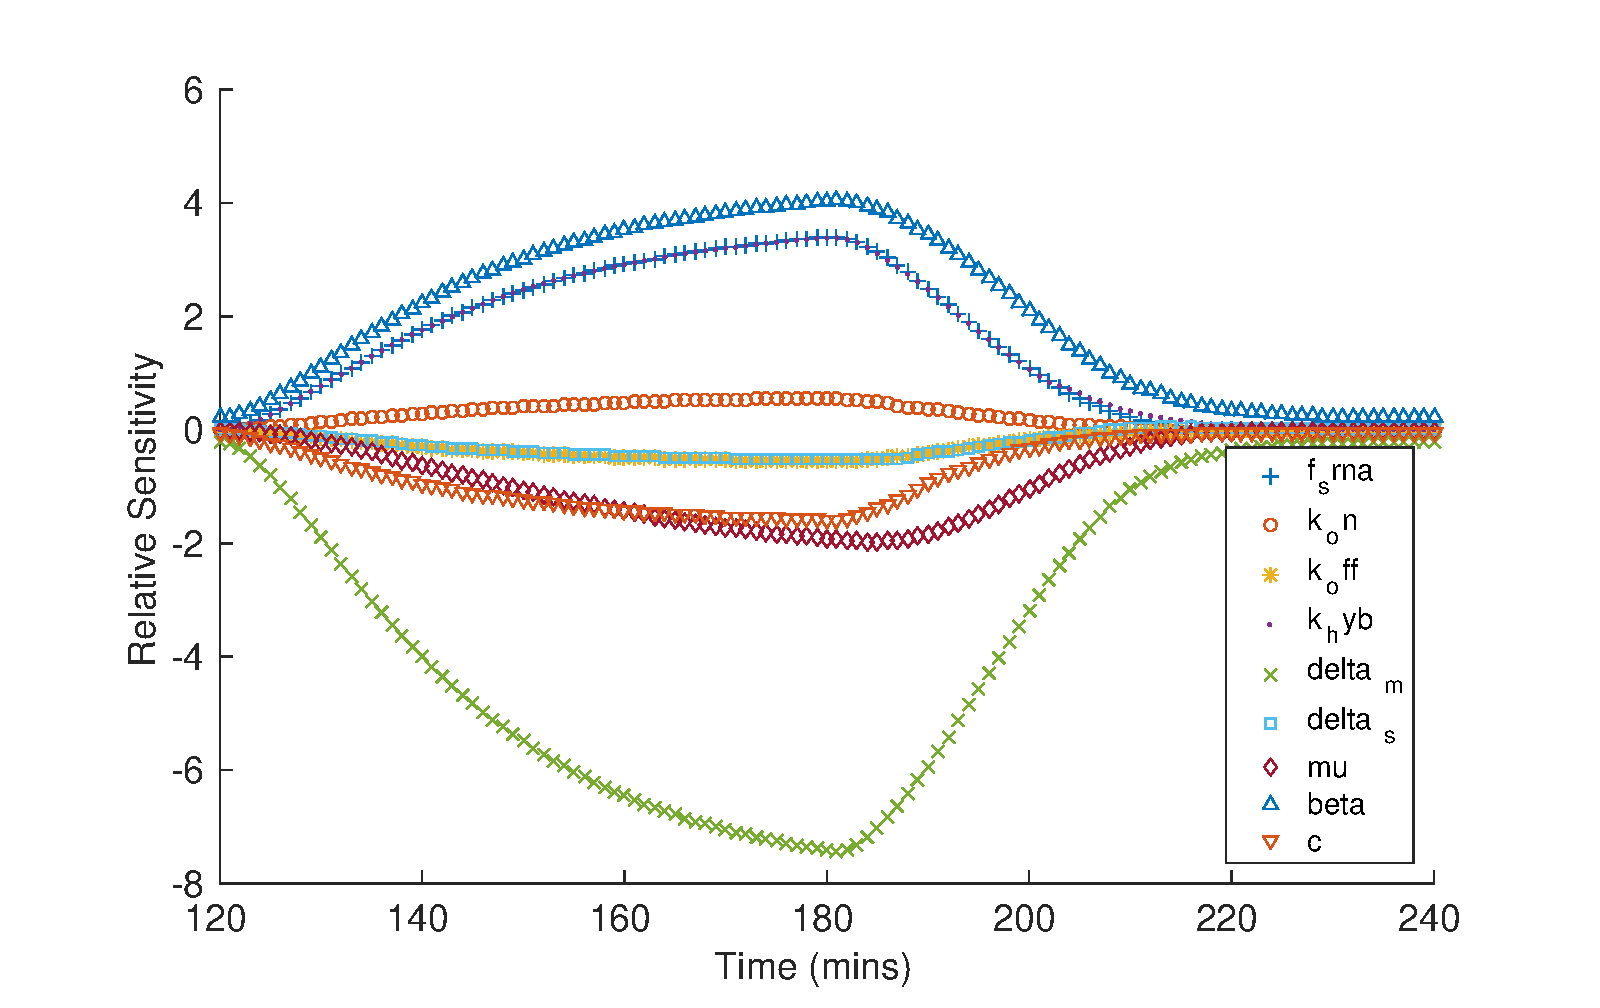
\includegraphics[scale = 0.3]{Sensitivity_unscaled}
        \caption{Unscaled}
        \label{SensitivityMatrix_unscaled} 
    \end{subfigure}
    \begin{subfigure}[h]{0.49\textwidth}
    \centering
        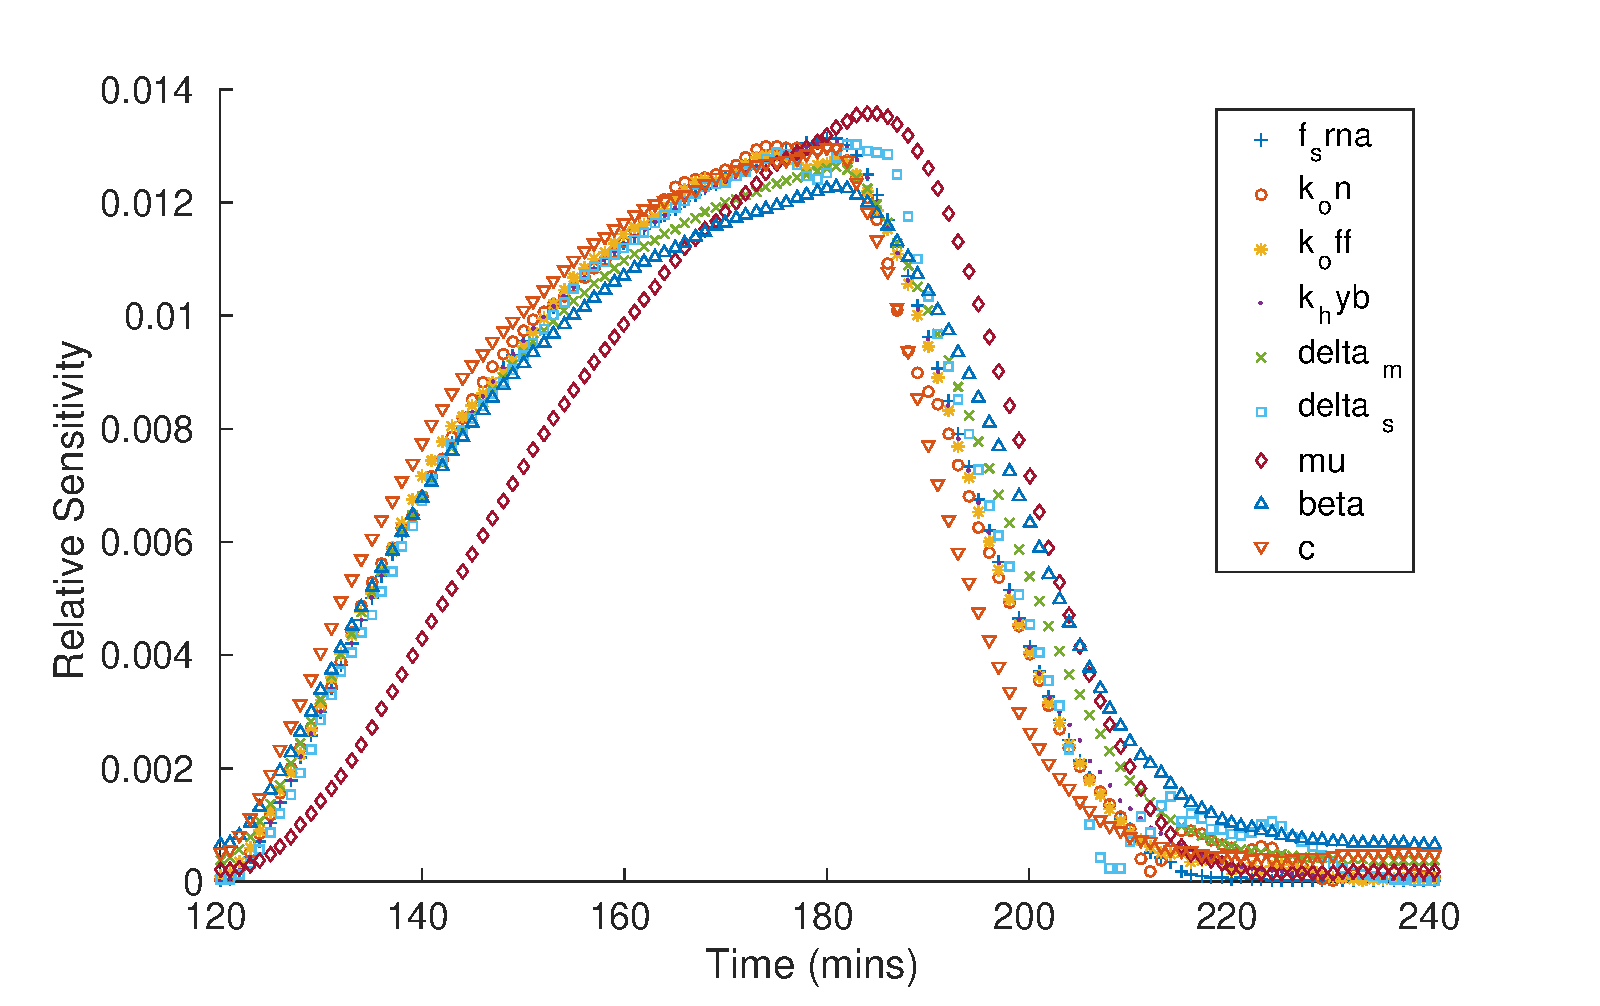
\includegraphics[scale = 0.3]{Sensitivity_scaled}
        \caption{Scaled}
                \label{SensitivityMatrix_scaled} 
    \end{subfigure}
    \caption{Sensitivity co-efficients $S_{ij}$ evaluated about a set of estimated parameters from the \textit{13\_9} dataset. \ref{SensitivityMatrix_unscaled} shows them unscaled, \ref{SensitivityMatrix_scaled} shows them scaled by the norm of each column of $S$.} 
\label{SensitivityMatrix}   
\end{figure}


 
 
 
 \begin{itemize}
 \item discuss estimatbility criteria- uniqeuess and sensitivity
 \item put in some sensitivity analysis results
 \item discuss model fixed points
 \item discuss systematic paramater shift.
 \item discuss cross - validation and predicitive ability of parameter sets found.
 \item suggest two times, work out fixed point for all the solutions found, look at structure of soln,
 \item re run from starting pararms.
 \end{itemize}
 
 
\begin{figure*}
    \begin{subfigure}[h]{0.49\textwidth}
    \centering
        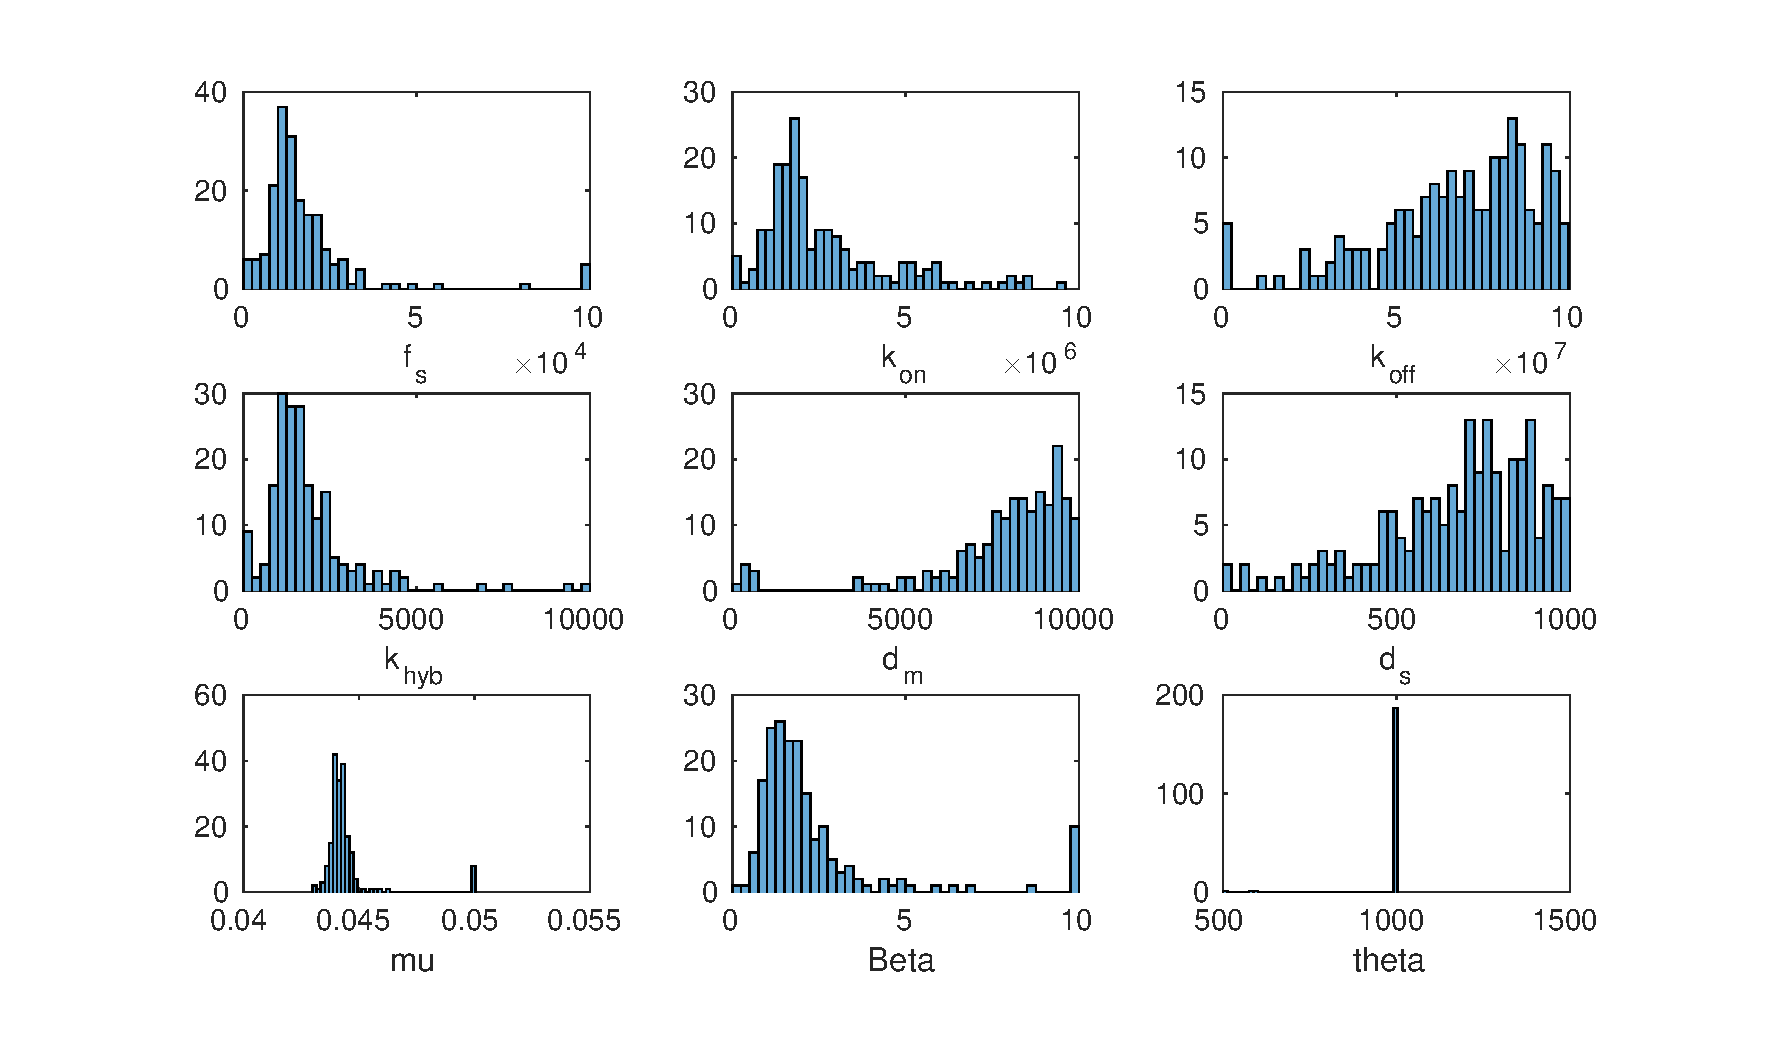
\includegraphics[scale = 0.35, clip = true, trim = 80 0 80 0]{13_9_hist.eps}
        \caption{Histogram of estimated parameter values, found from 200 runs of the CMA-ES algorithm. Fitted to the \textit{13\_9} dataset. }
    \end{subfigure}
    \begin{subfigure}[c]{0.49\textwidth}
    \centering
        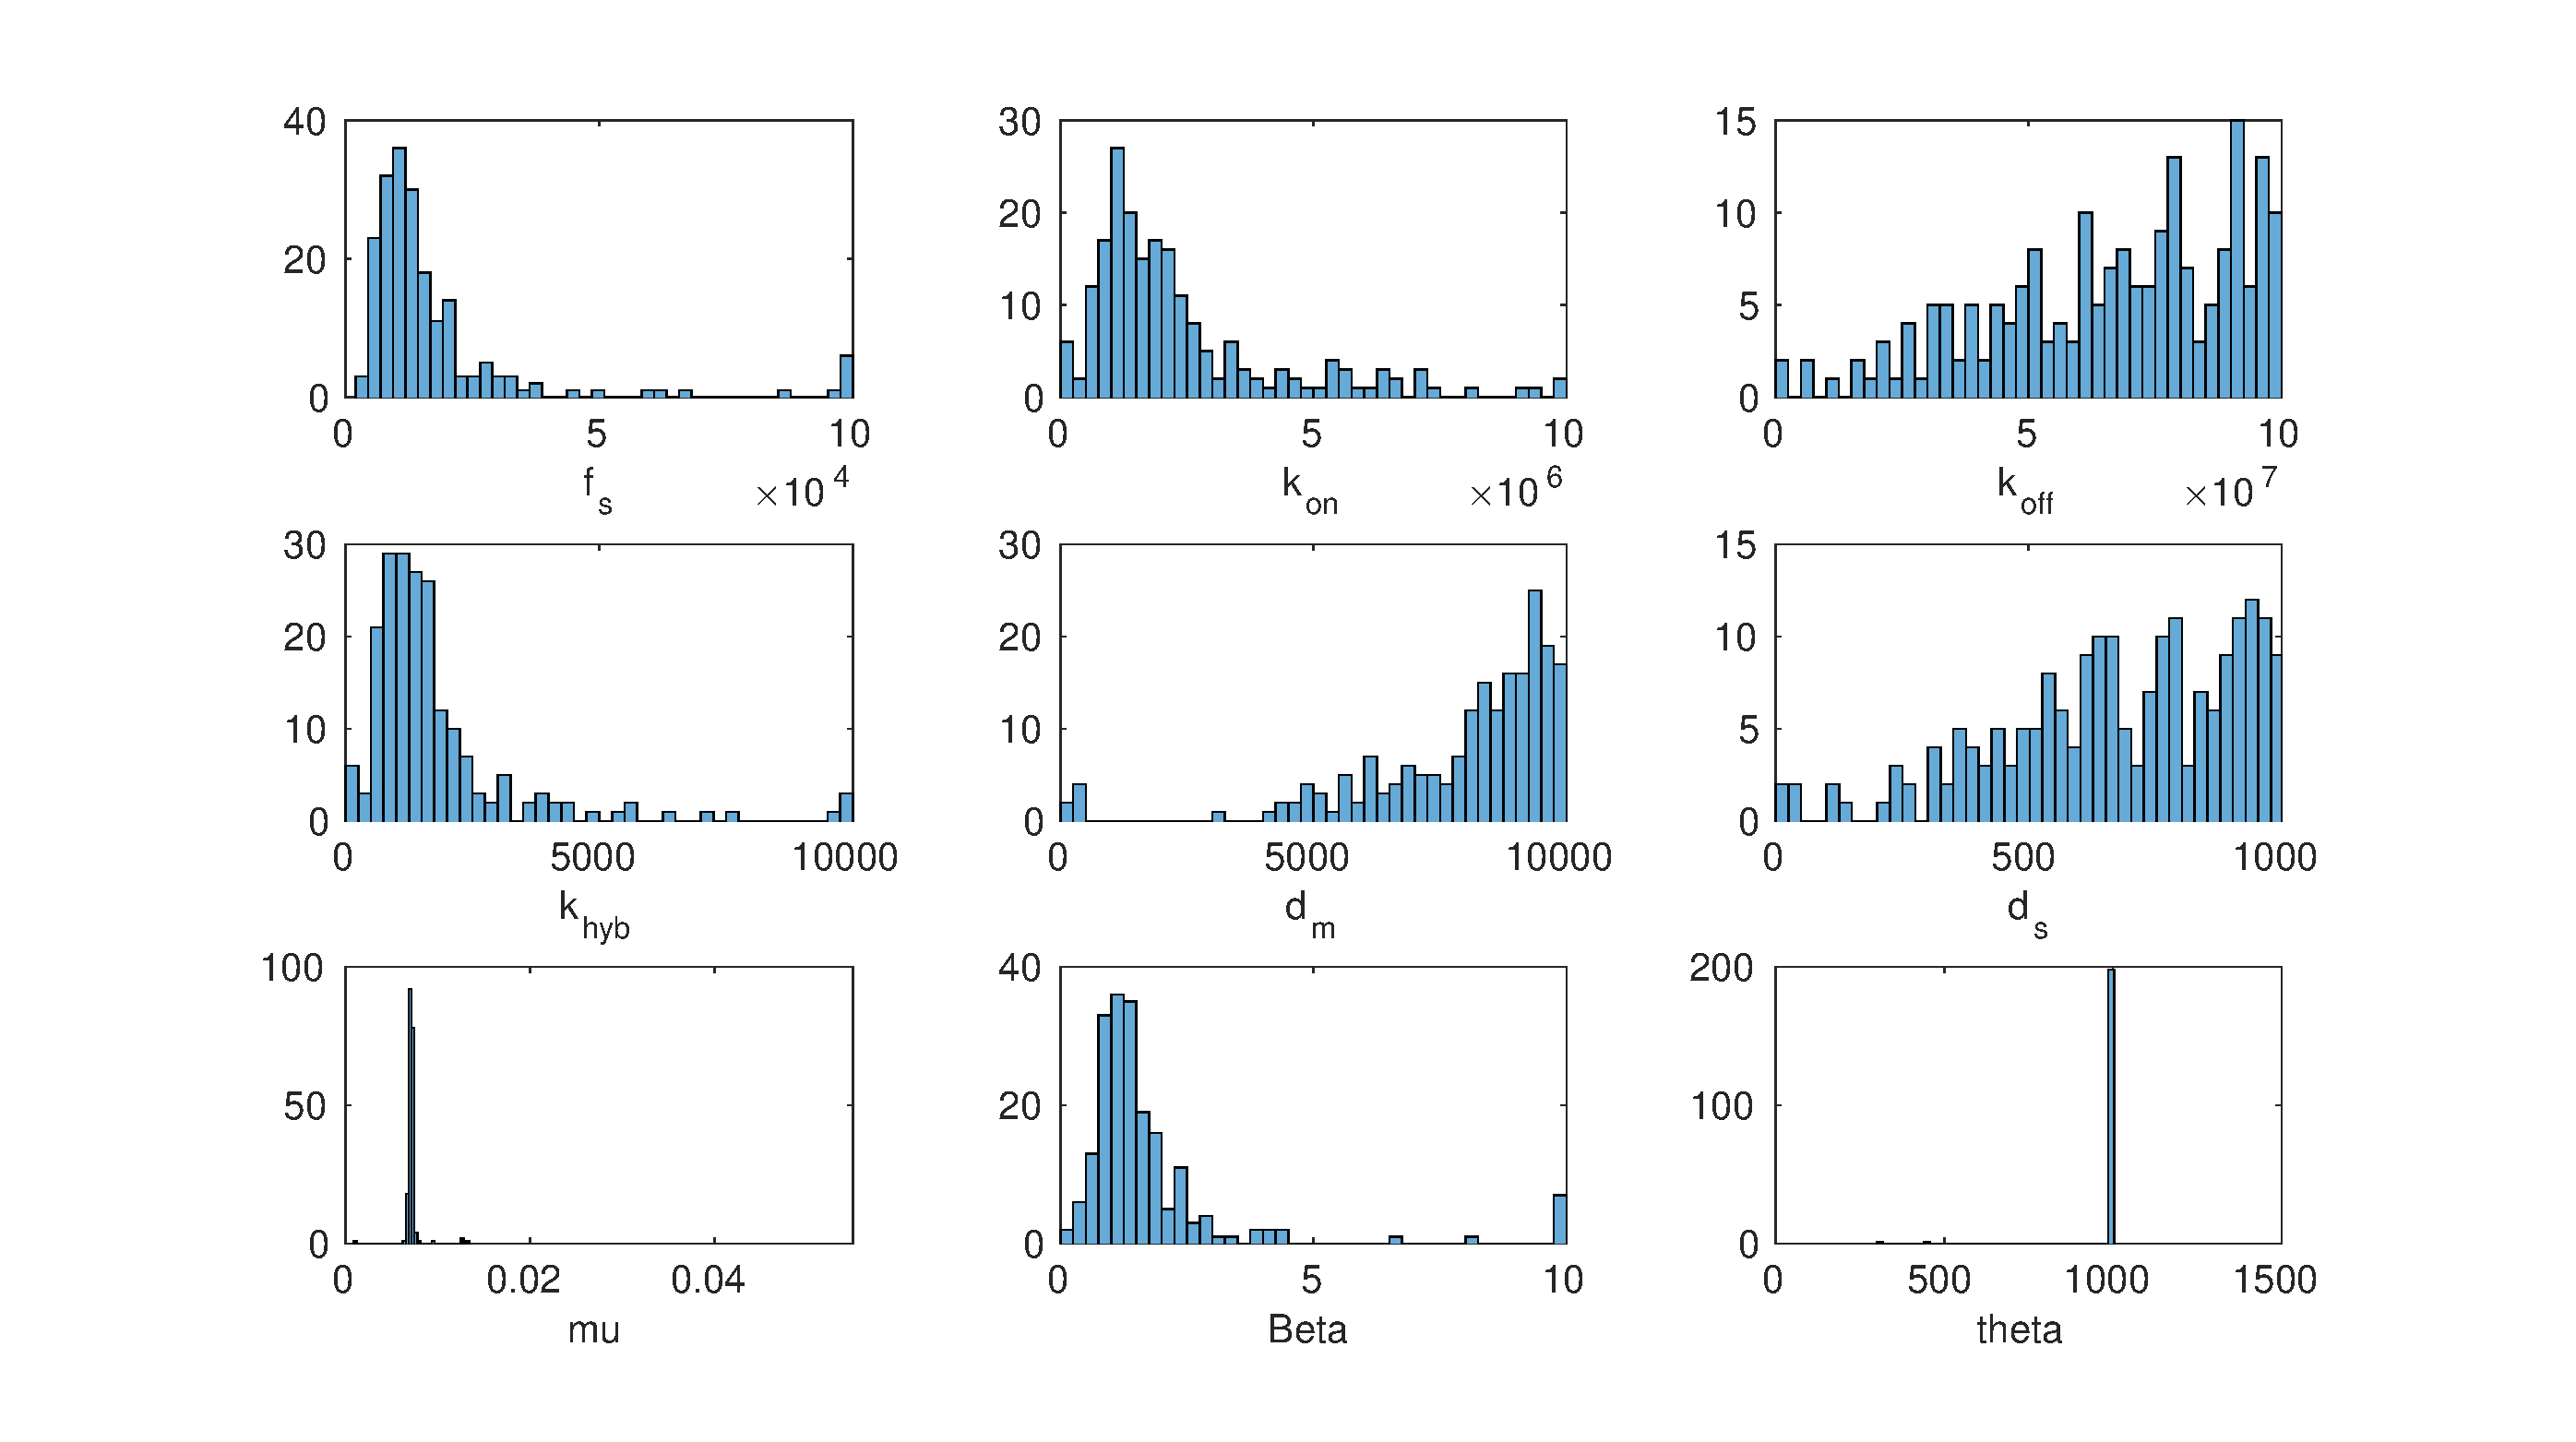
\includegraphics[scale = 0.38,clip = true, trim = 60 12 80 0]{14_7_hist.eps}
        \caption{Histogram of estimated parameter values, found from 200 runs of the CMA-ES algorithm. Fitted to the \textit{14\_7} dataset. }
    \end{subfigure}

        \begin{subfigure}[c]{0.49\textwidth}
        \centering
    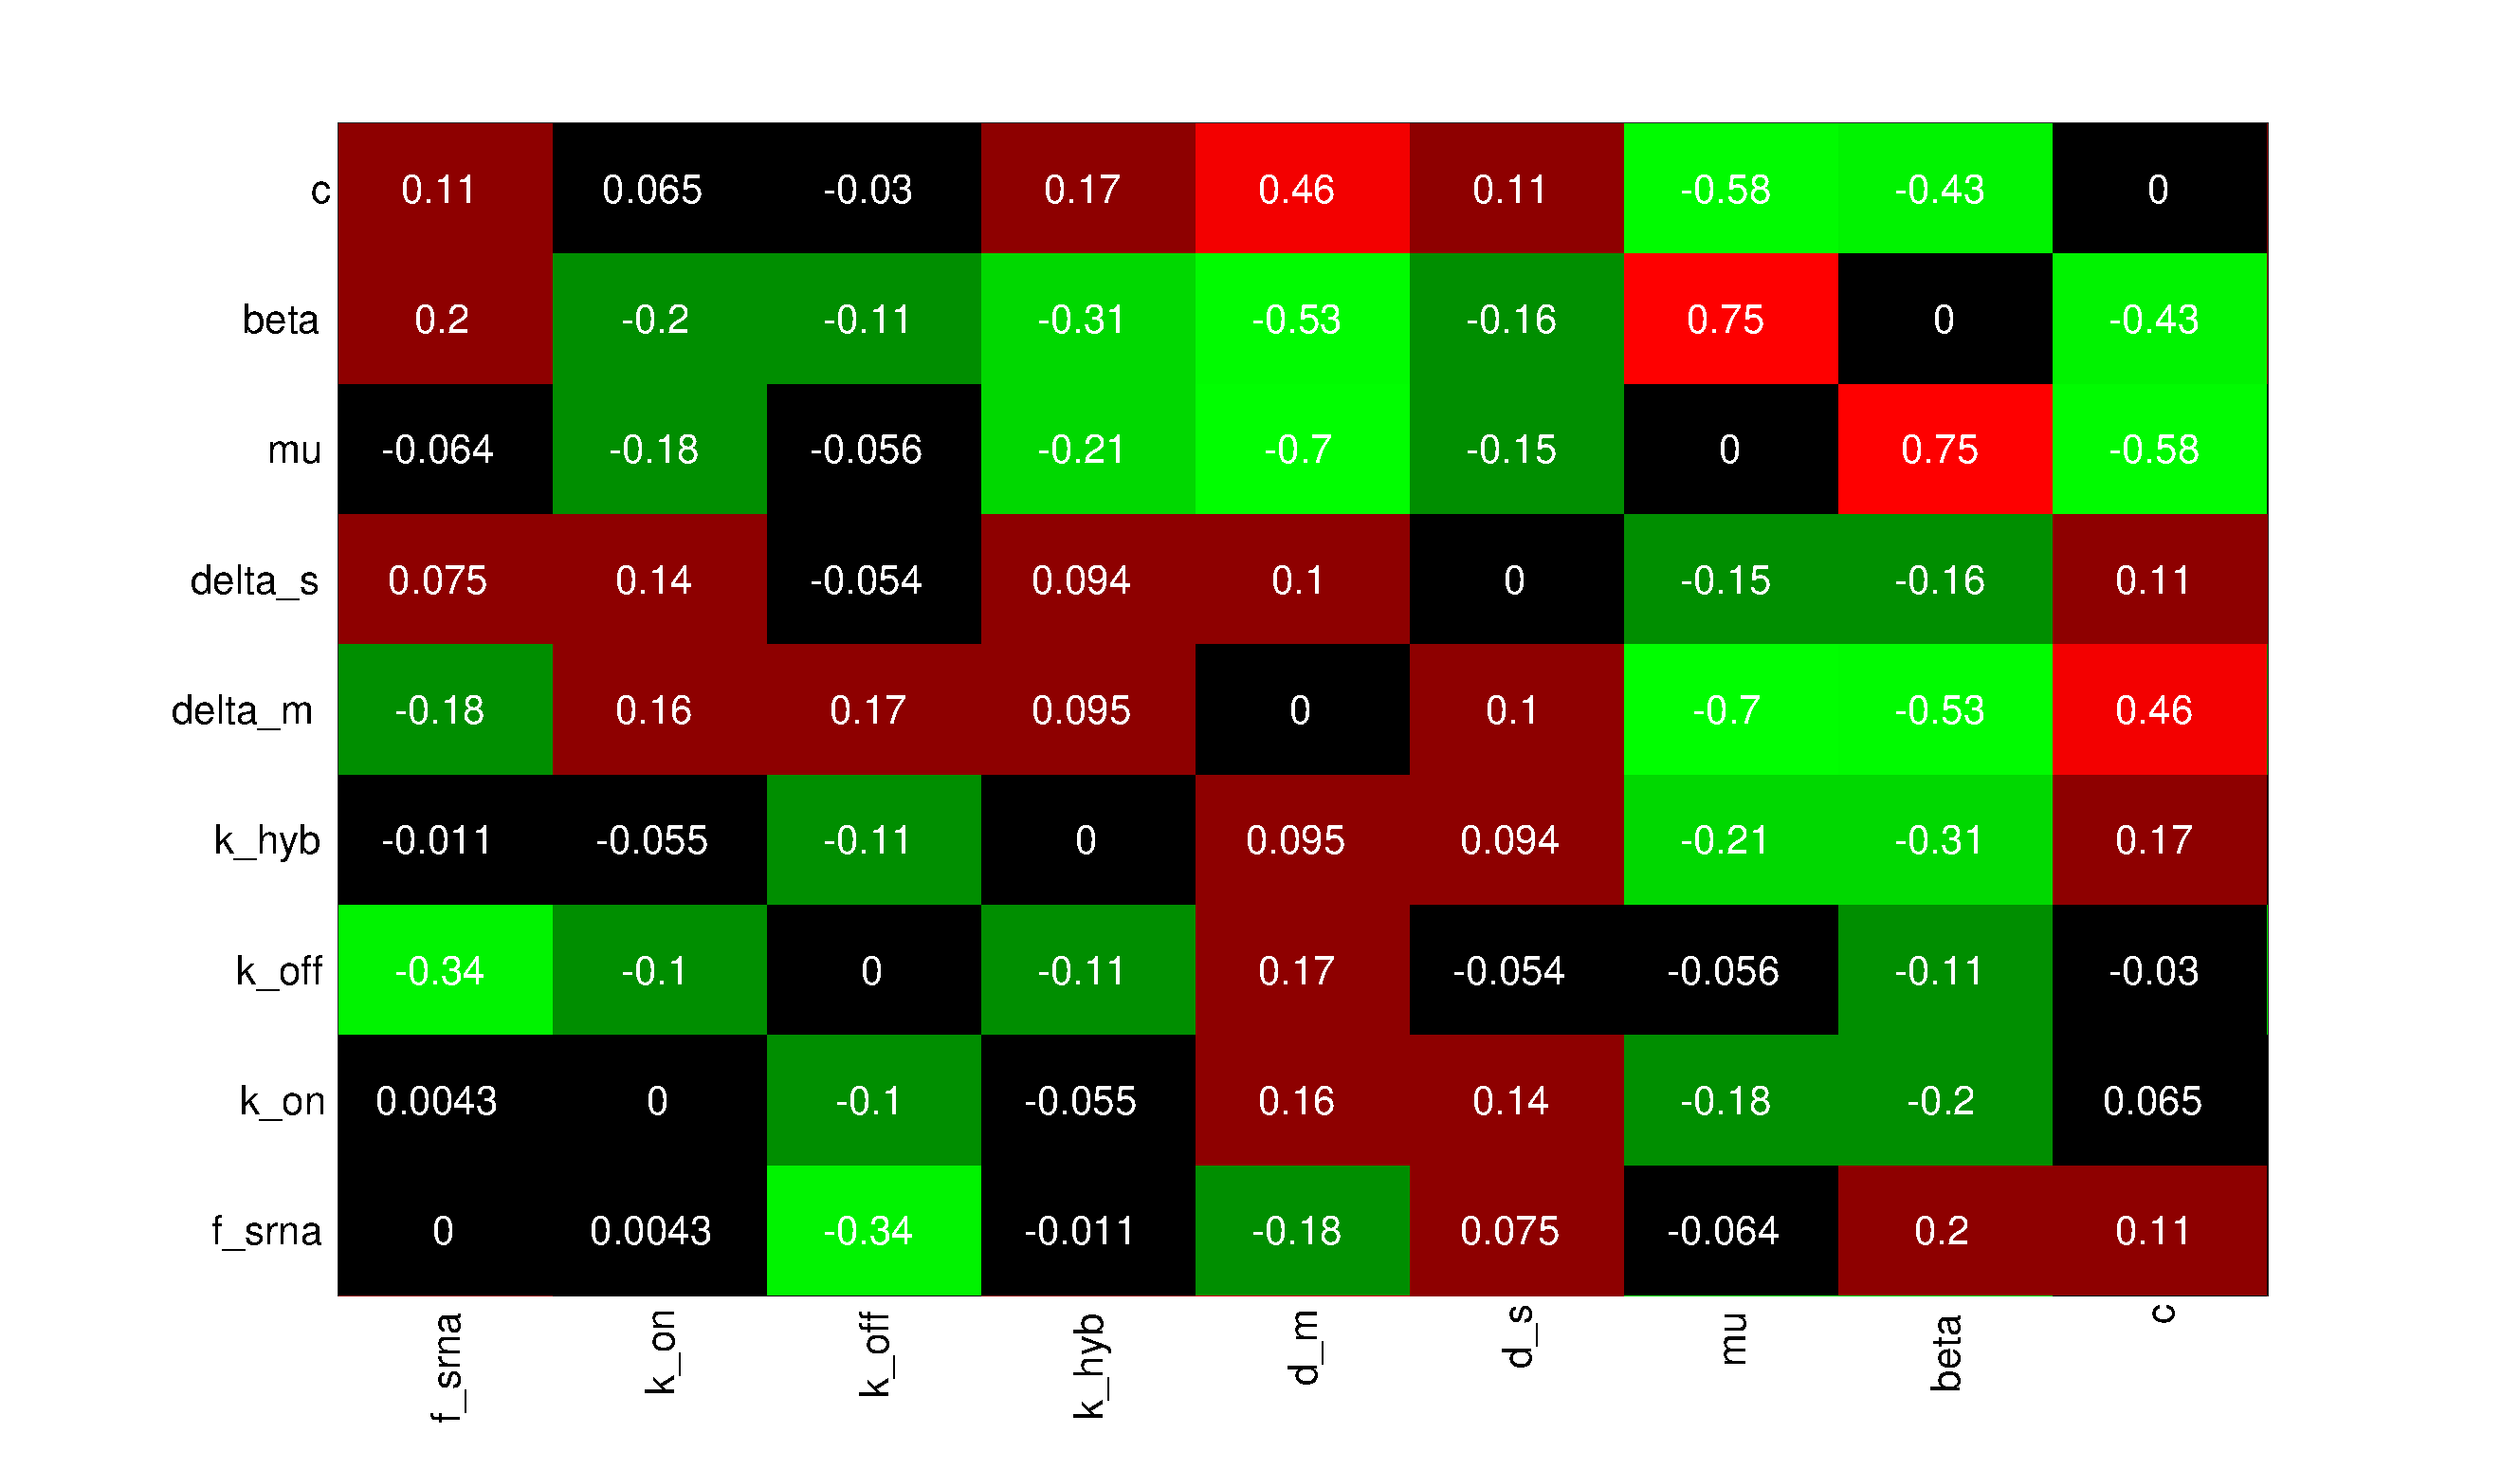
\includegraphics[scale = 0.25, clip = true, trim = 100 0 100 0]{13_9_heatmap.eps}
        \caption{Correlation matrix of estimated parameter sets, from the  \textit{13\_9} dataset. }
    \end{subfigure}
    \begin{subfigure}[c]{0.49\textwidth}
    \centering
        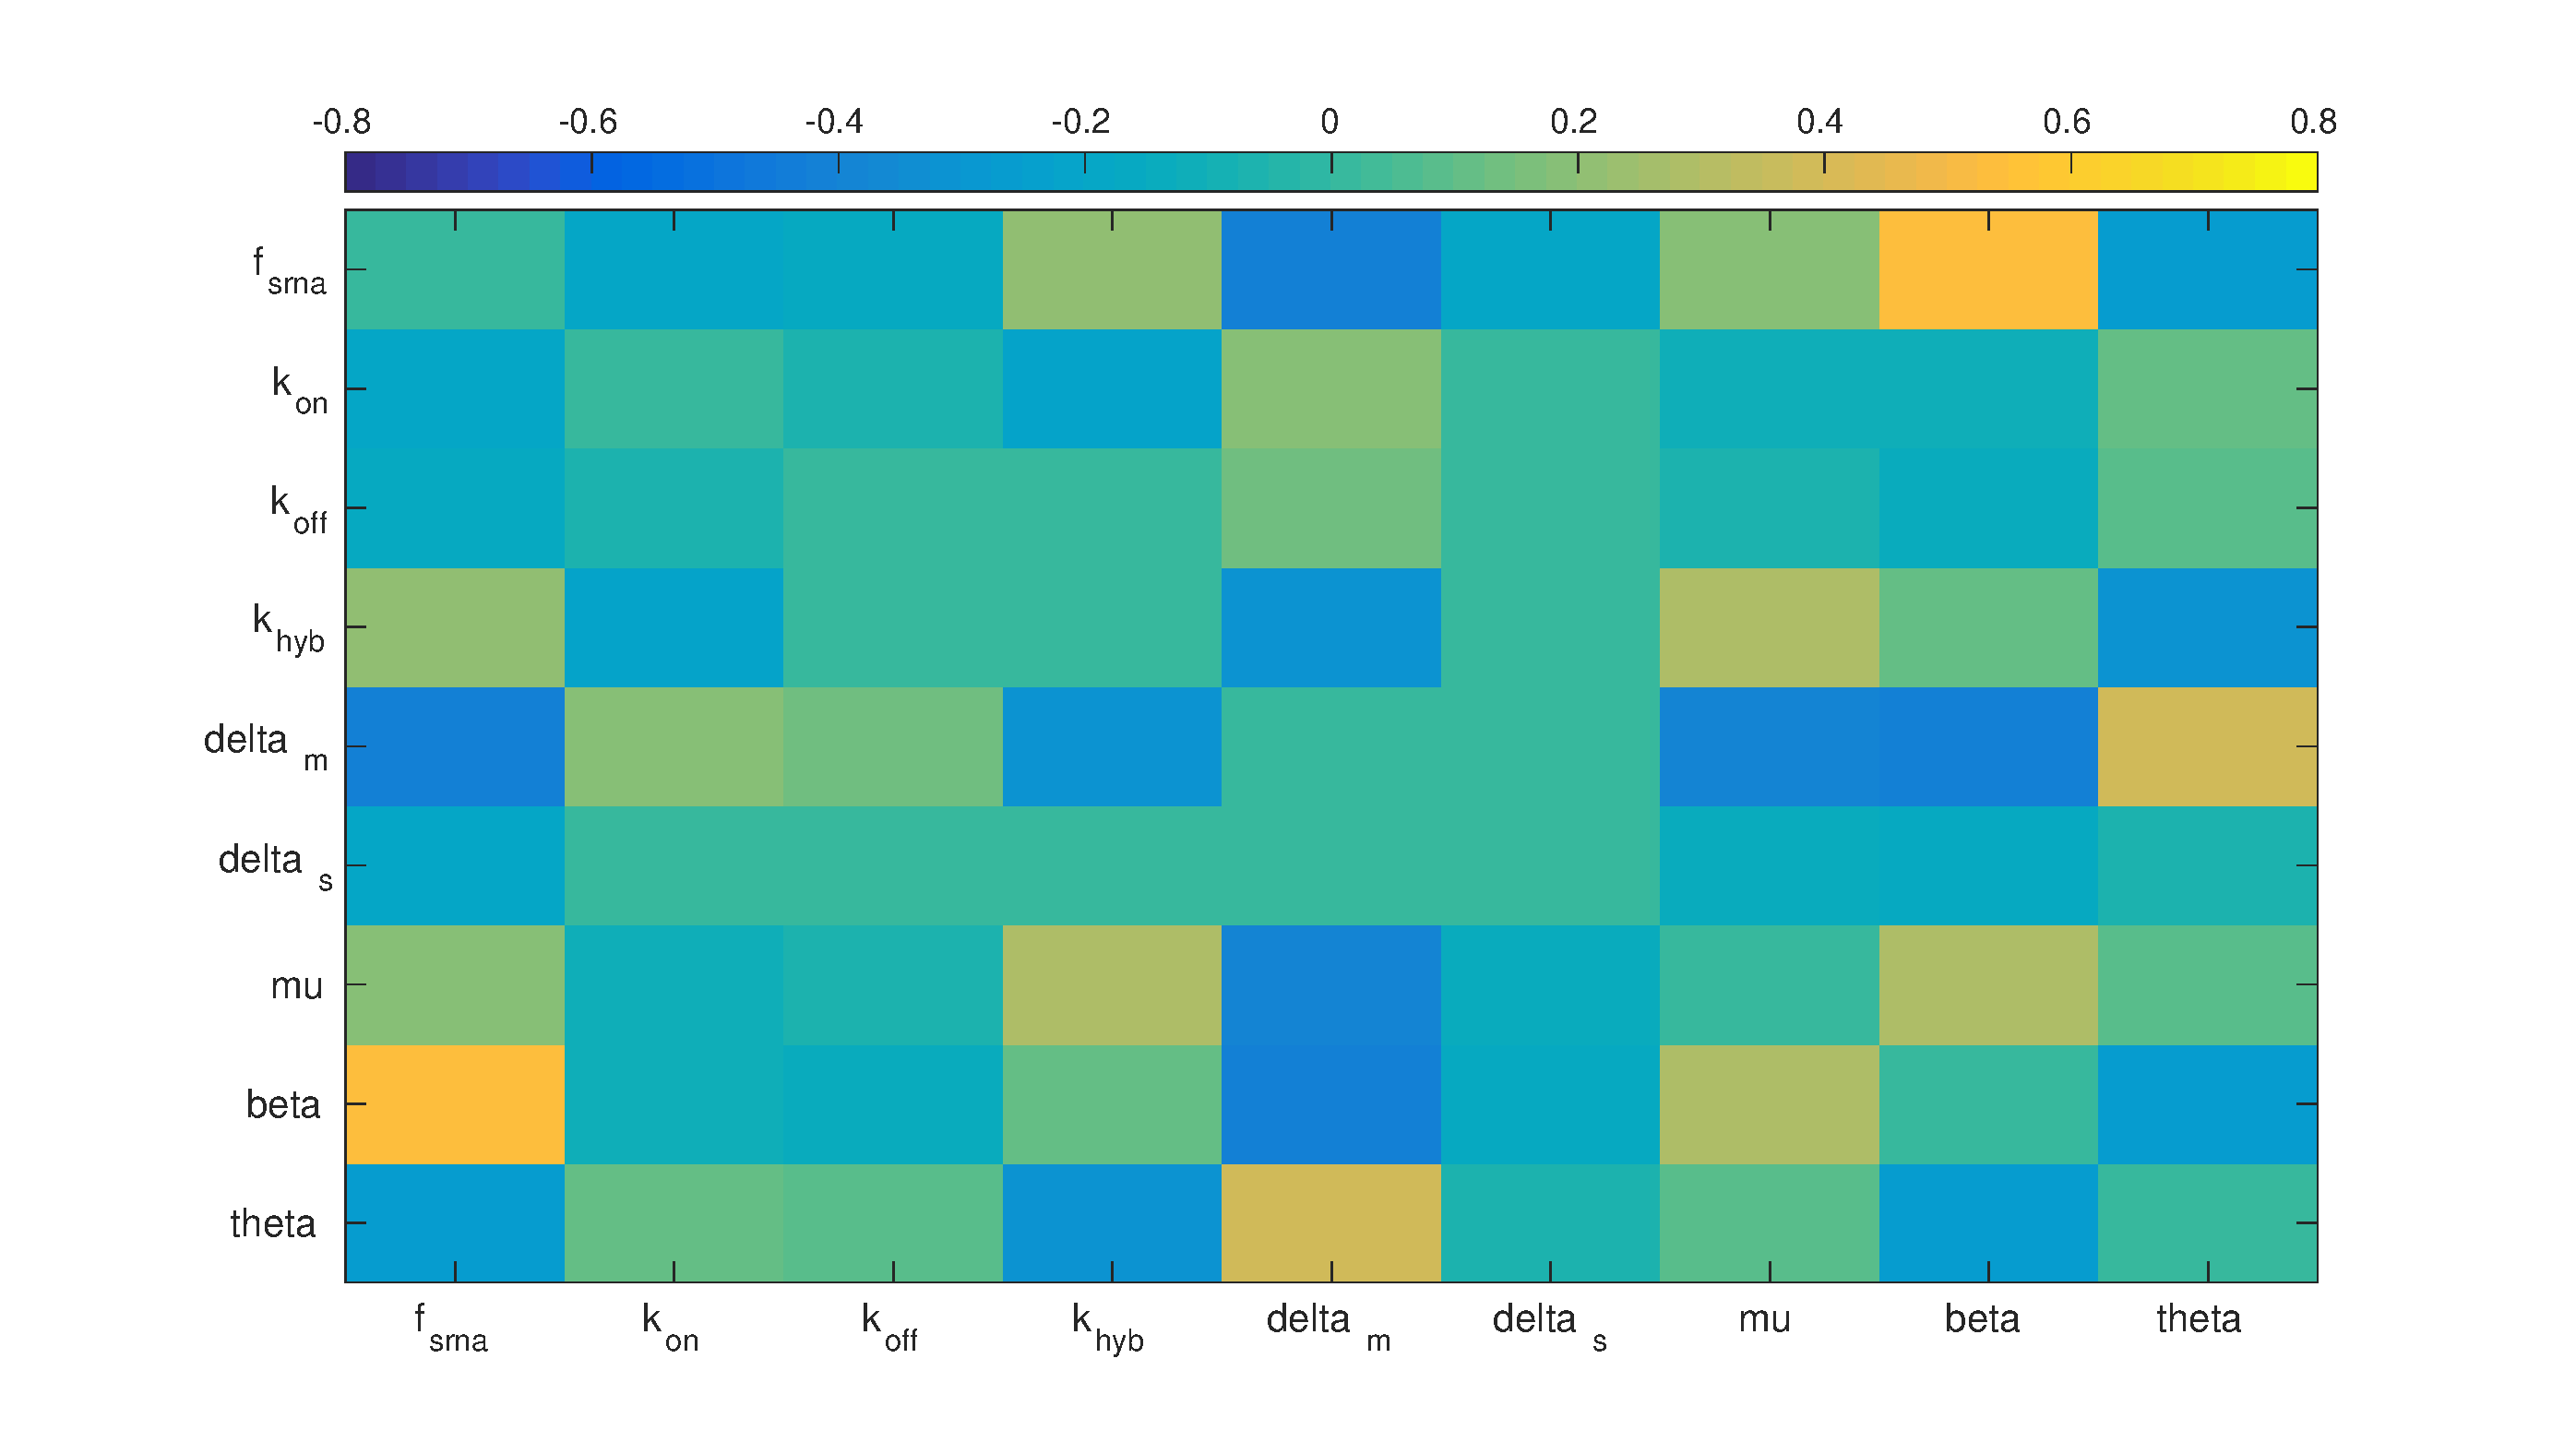
\includegraphics[scale = 0.25, clip = true, trim = 80 0 80 0]{14_7_heatmap.eps}
        \caption{Correlation matrix of estimated parameter sets, from the  \textit{14\_7} dataset.}
    \end{subfigure}
    
    \begin{subfigure}[c]{0.49\textwidth}
    \centering
    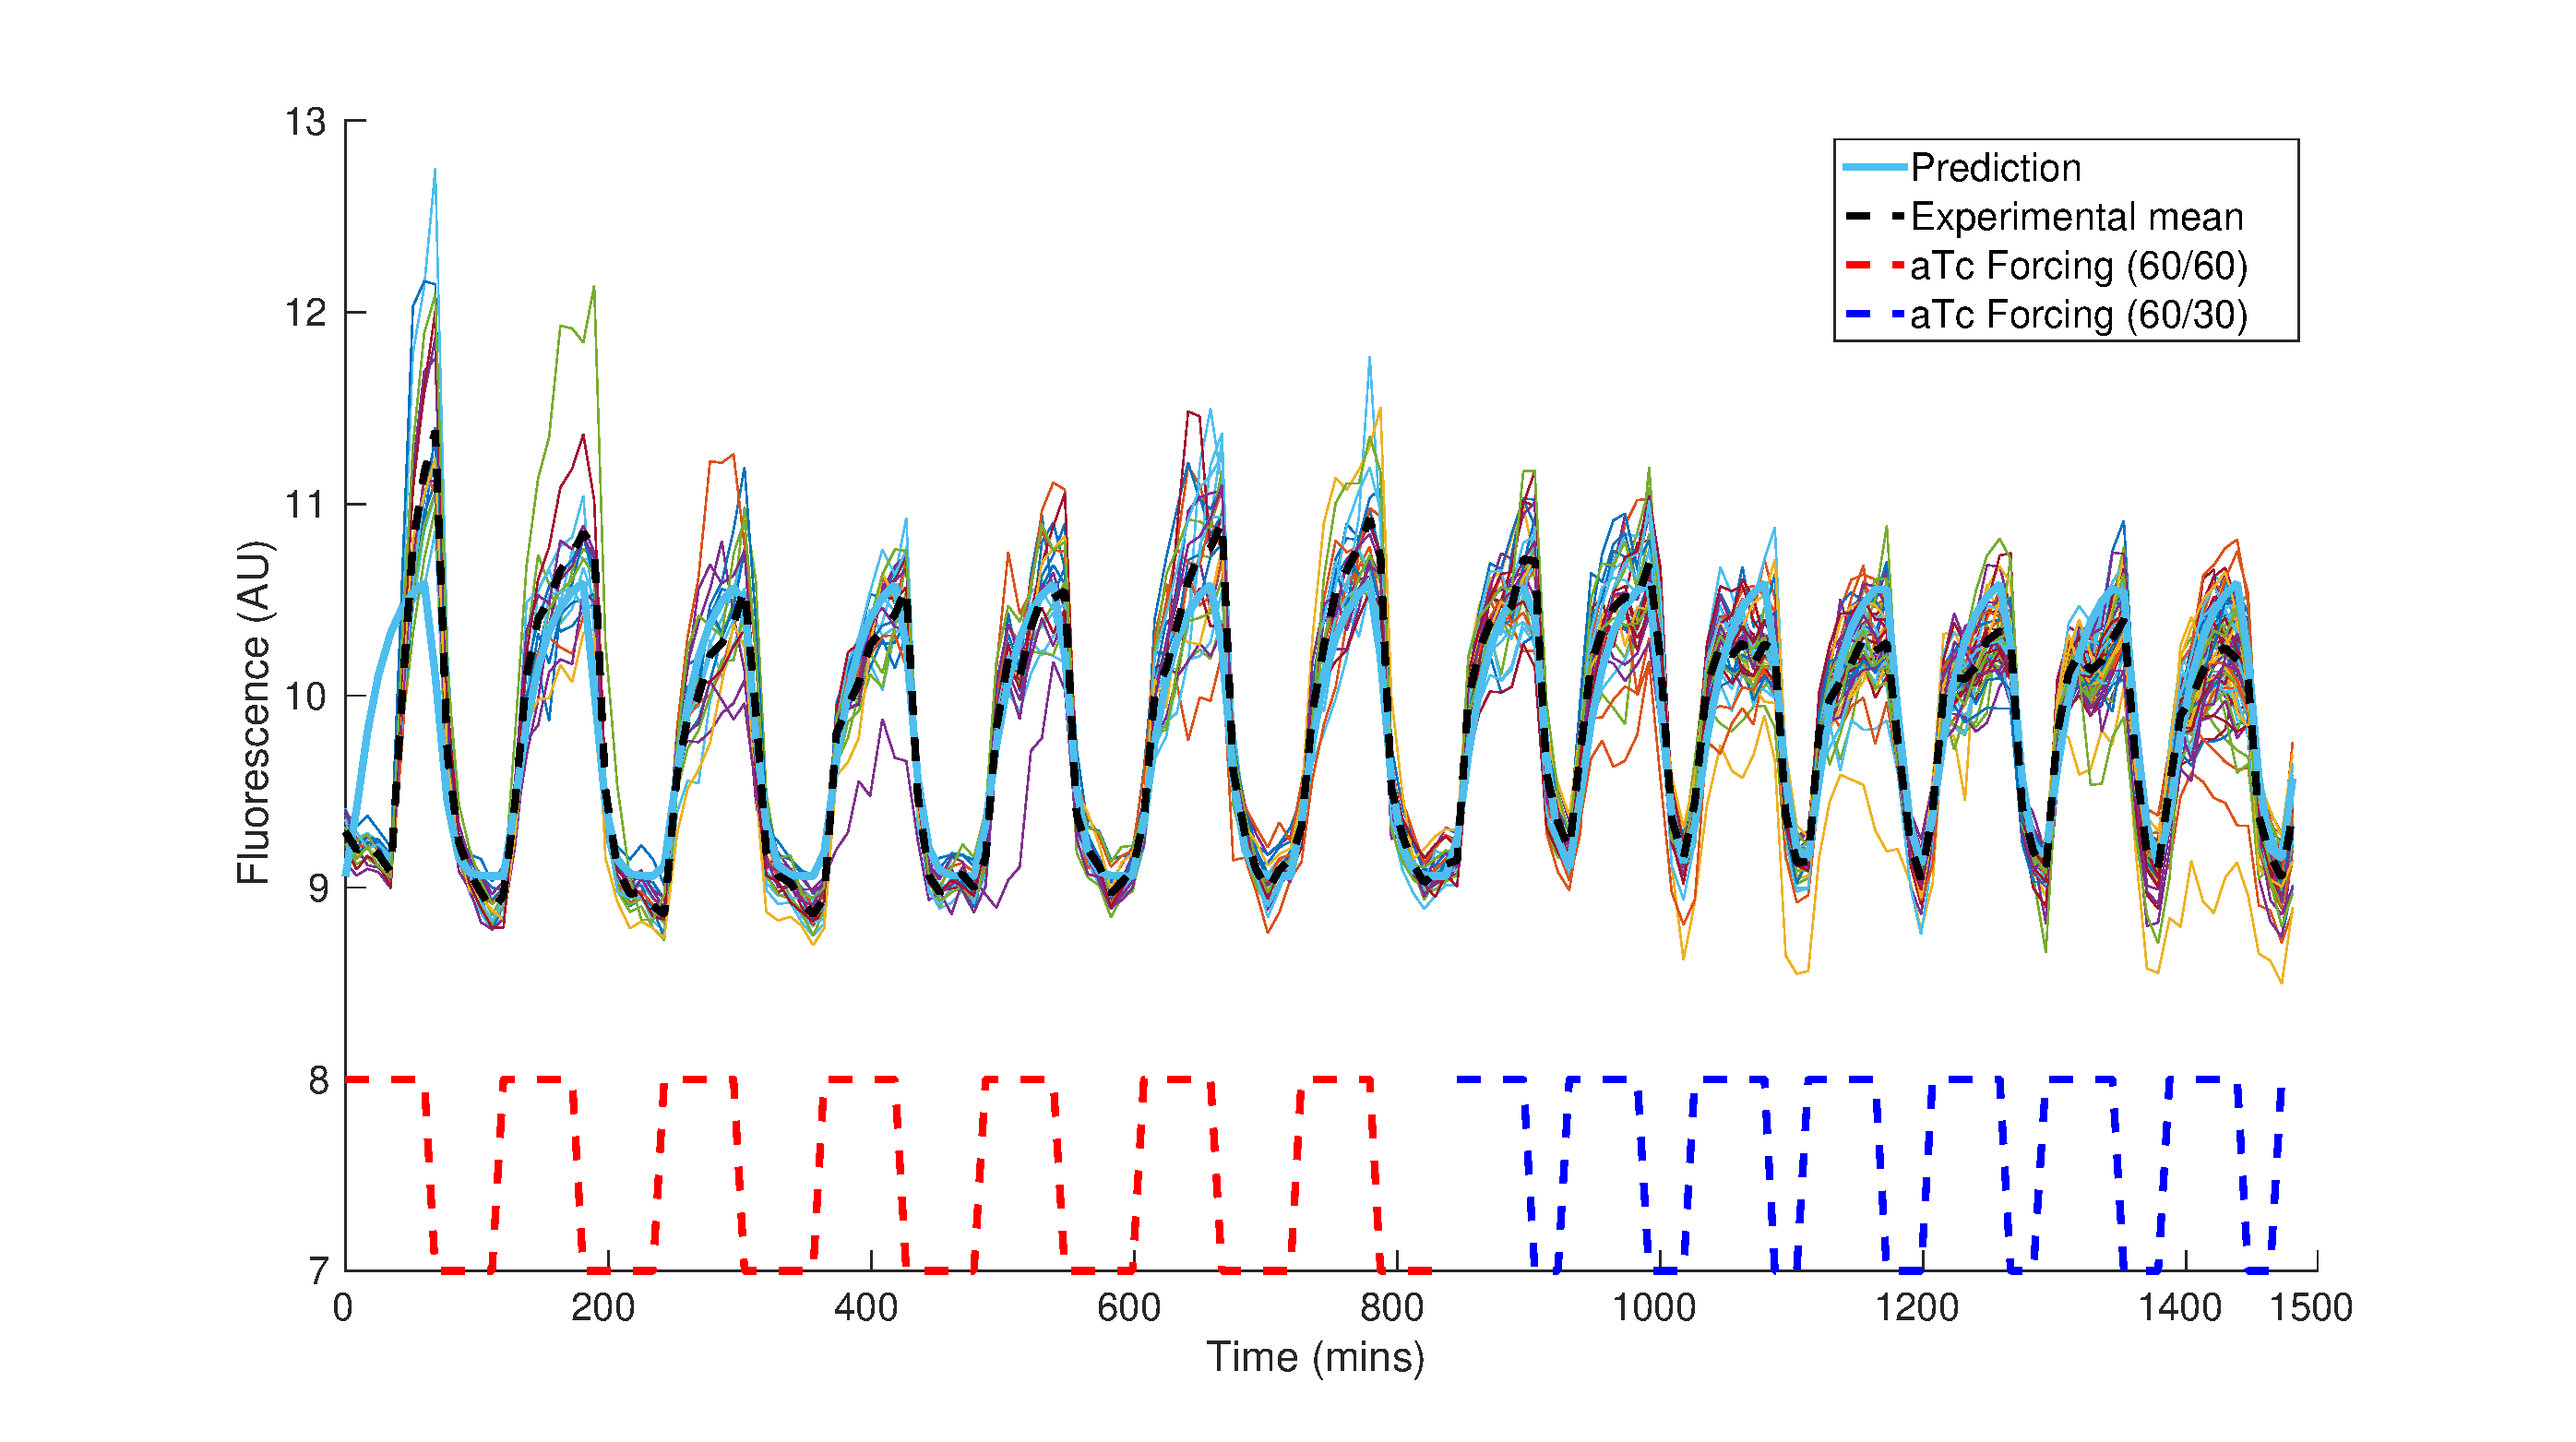
\includegraphics[scale = 0.37]{13_9_bestPlot}
        \caption{Model prediction, using the parameter set with the smallest error value of the initial 200 found, for the \textit{13\_9} dataset. A}
    \end{subfigure}
    \begin{subfigure}[c]{0.49\textwidth}
    \centering
        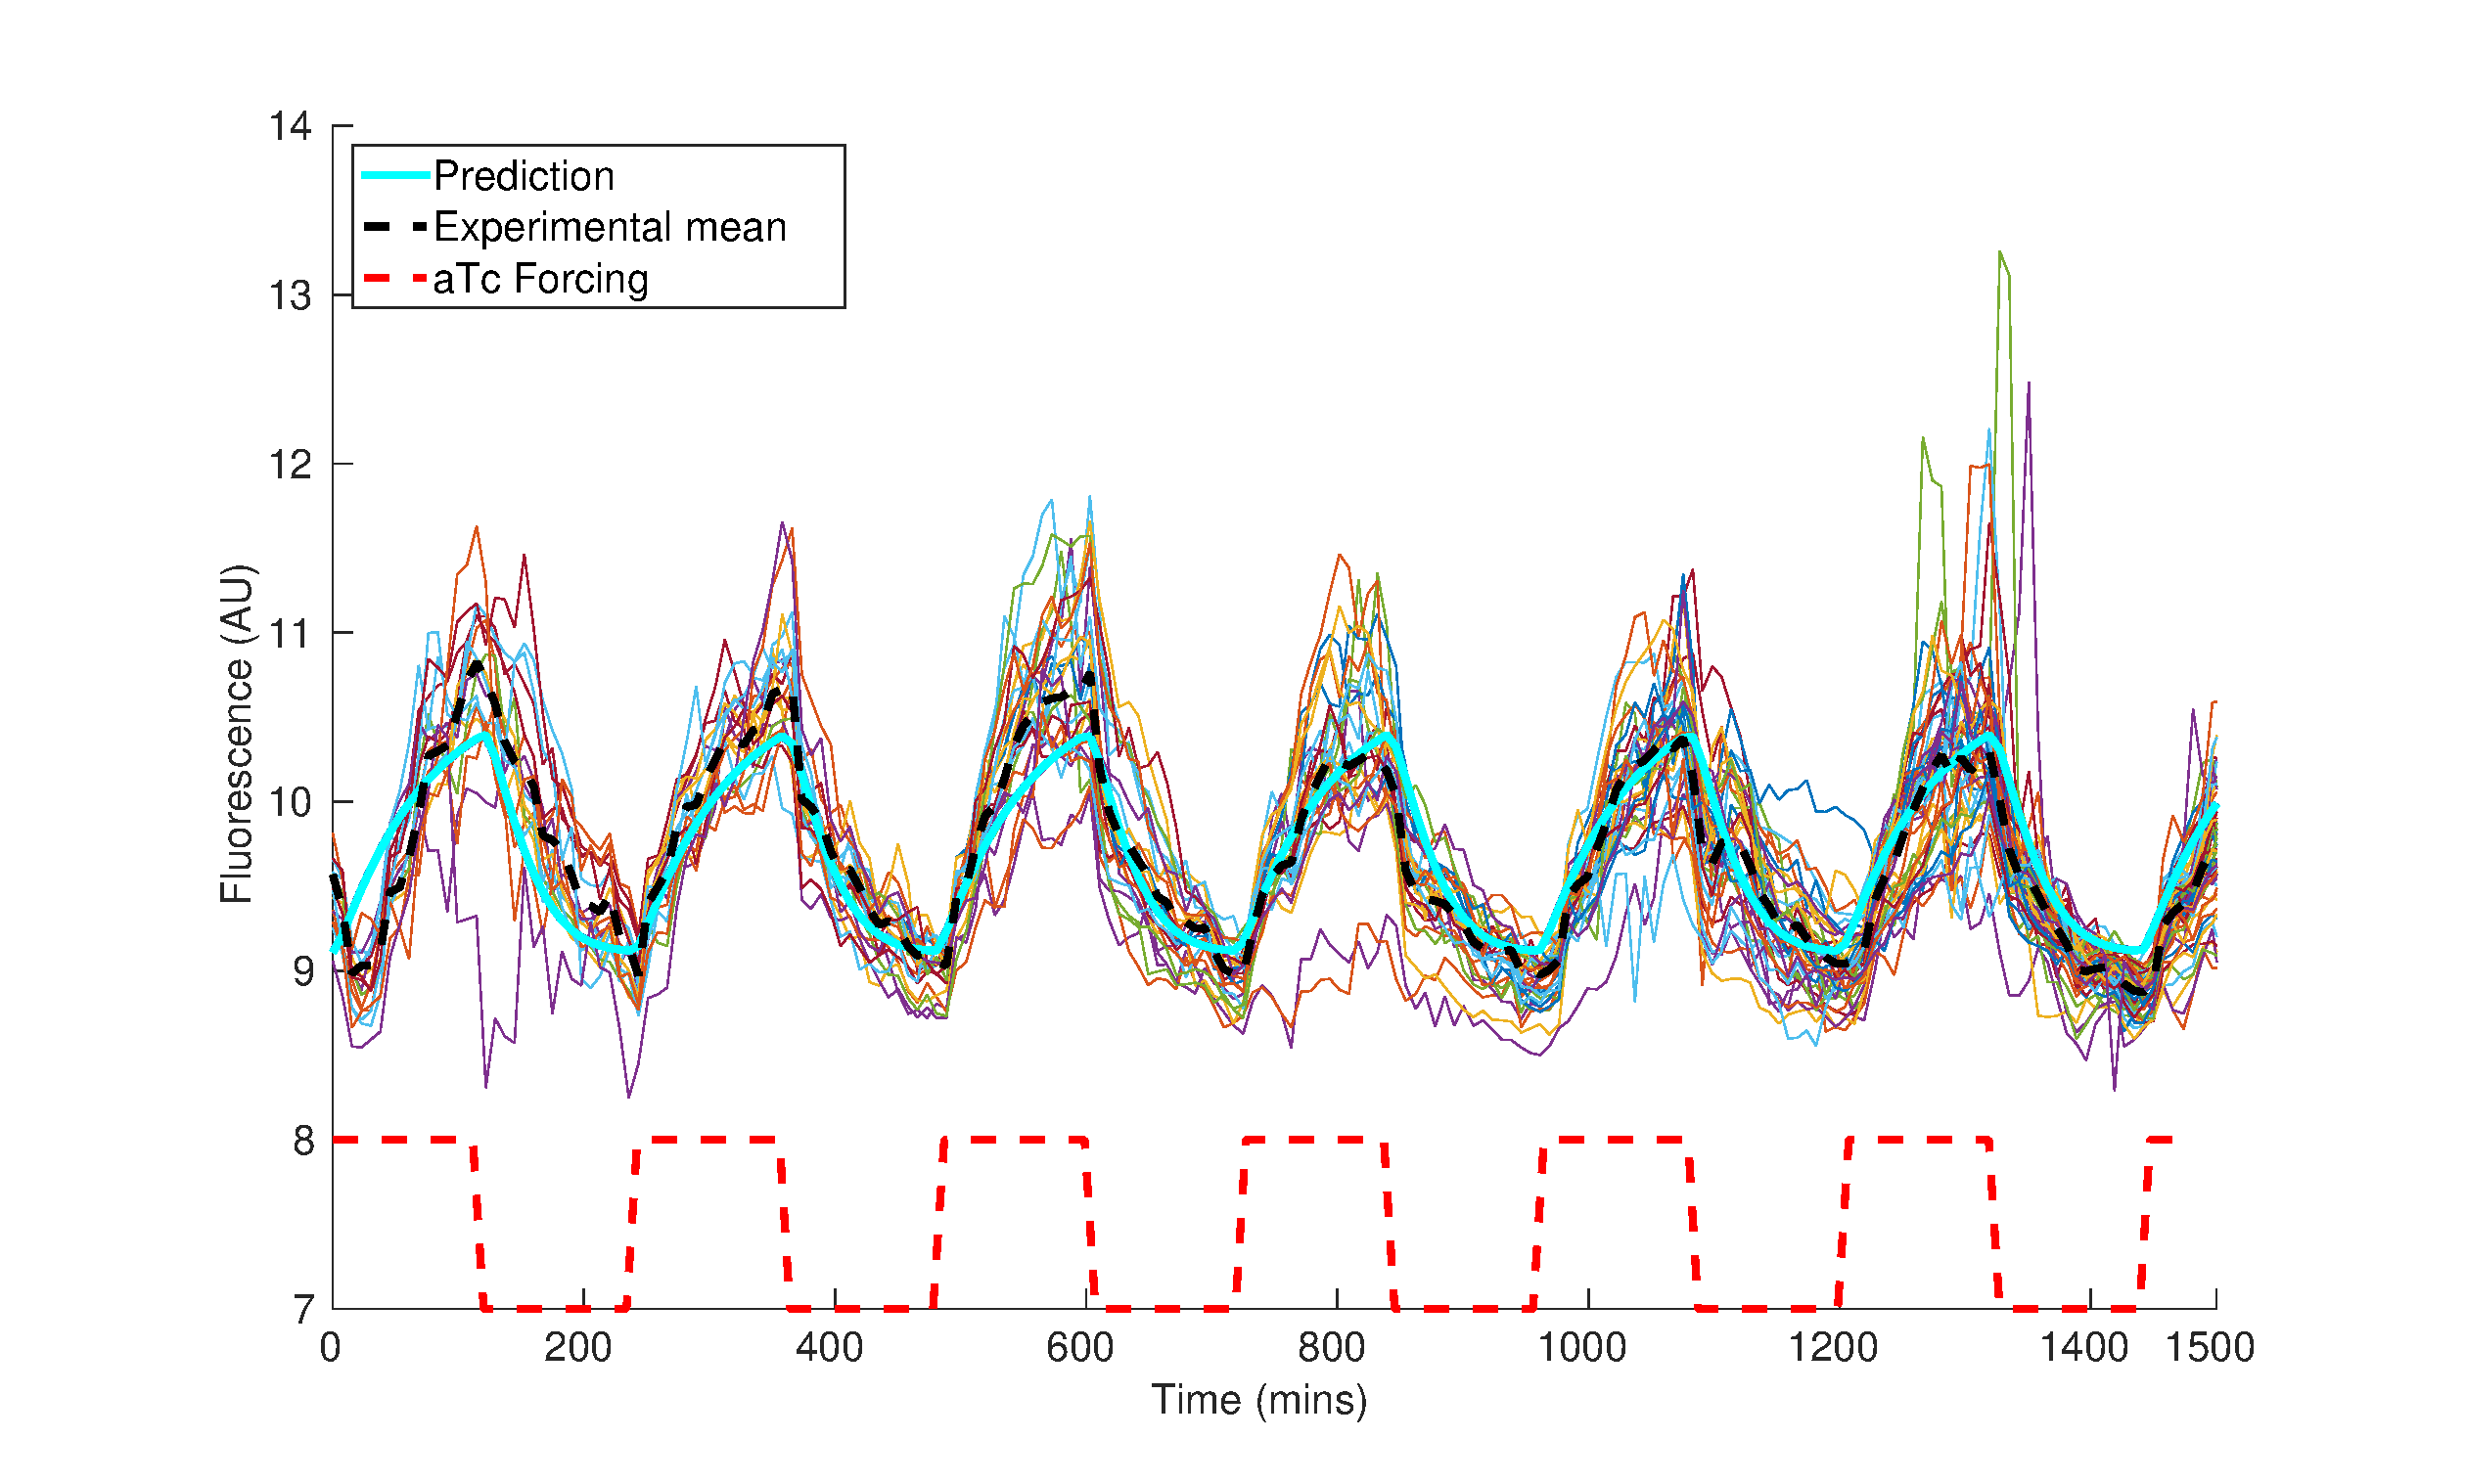
\includegraphics[scale = 0.37]{14_7_bestPlot}
        \caption{Model prediction, using the parameter set with the smallest error value of the initial 200 found, for the \textit{14\_7} dataset.}
    \end{subfigure}
    \caption{Parameter estimates, inter-parameter correlation values, and model predictions for the \textit{13\_9} and \textit{14\_7} datasets. Note that in the model predictions, aTc forcing is shown - IPTG concentration is constant at a level which saturates the cell's response. The forcing curve's height is schematic - aTc concentration is switched between off, and a level which saturates the cell's response}
\label{InitialResults}
\end{figure*} 
 


\clearpage
 

\section{Conclusions and Further work}
\label{Conclusions and Further work}

\todo[inline]{some stuff}

% references section
\bibliographystyle{./IEEE_bibtex_class/IEEEtran}
\bibliography{./IEEE_bibtex_class/IEEEabrv,library}

\clearpage
\onecolumn

\appendices
\renewcommand\thefigure{\thesection.\arabic{figure}}  


\section{Initial Experimental Data}
\label{Initial Experimental Data}
\setcounter{figure}{0}    

\begin{figure}[h]
\centering
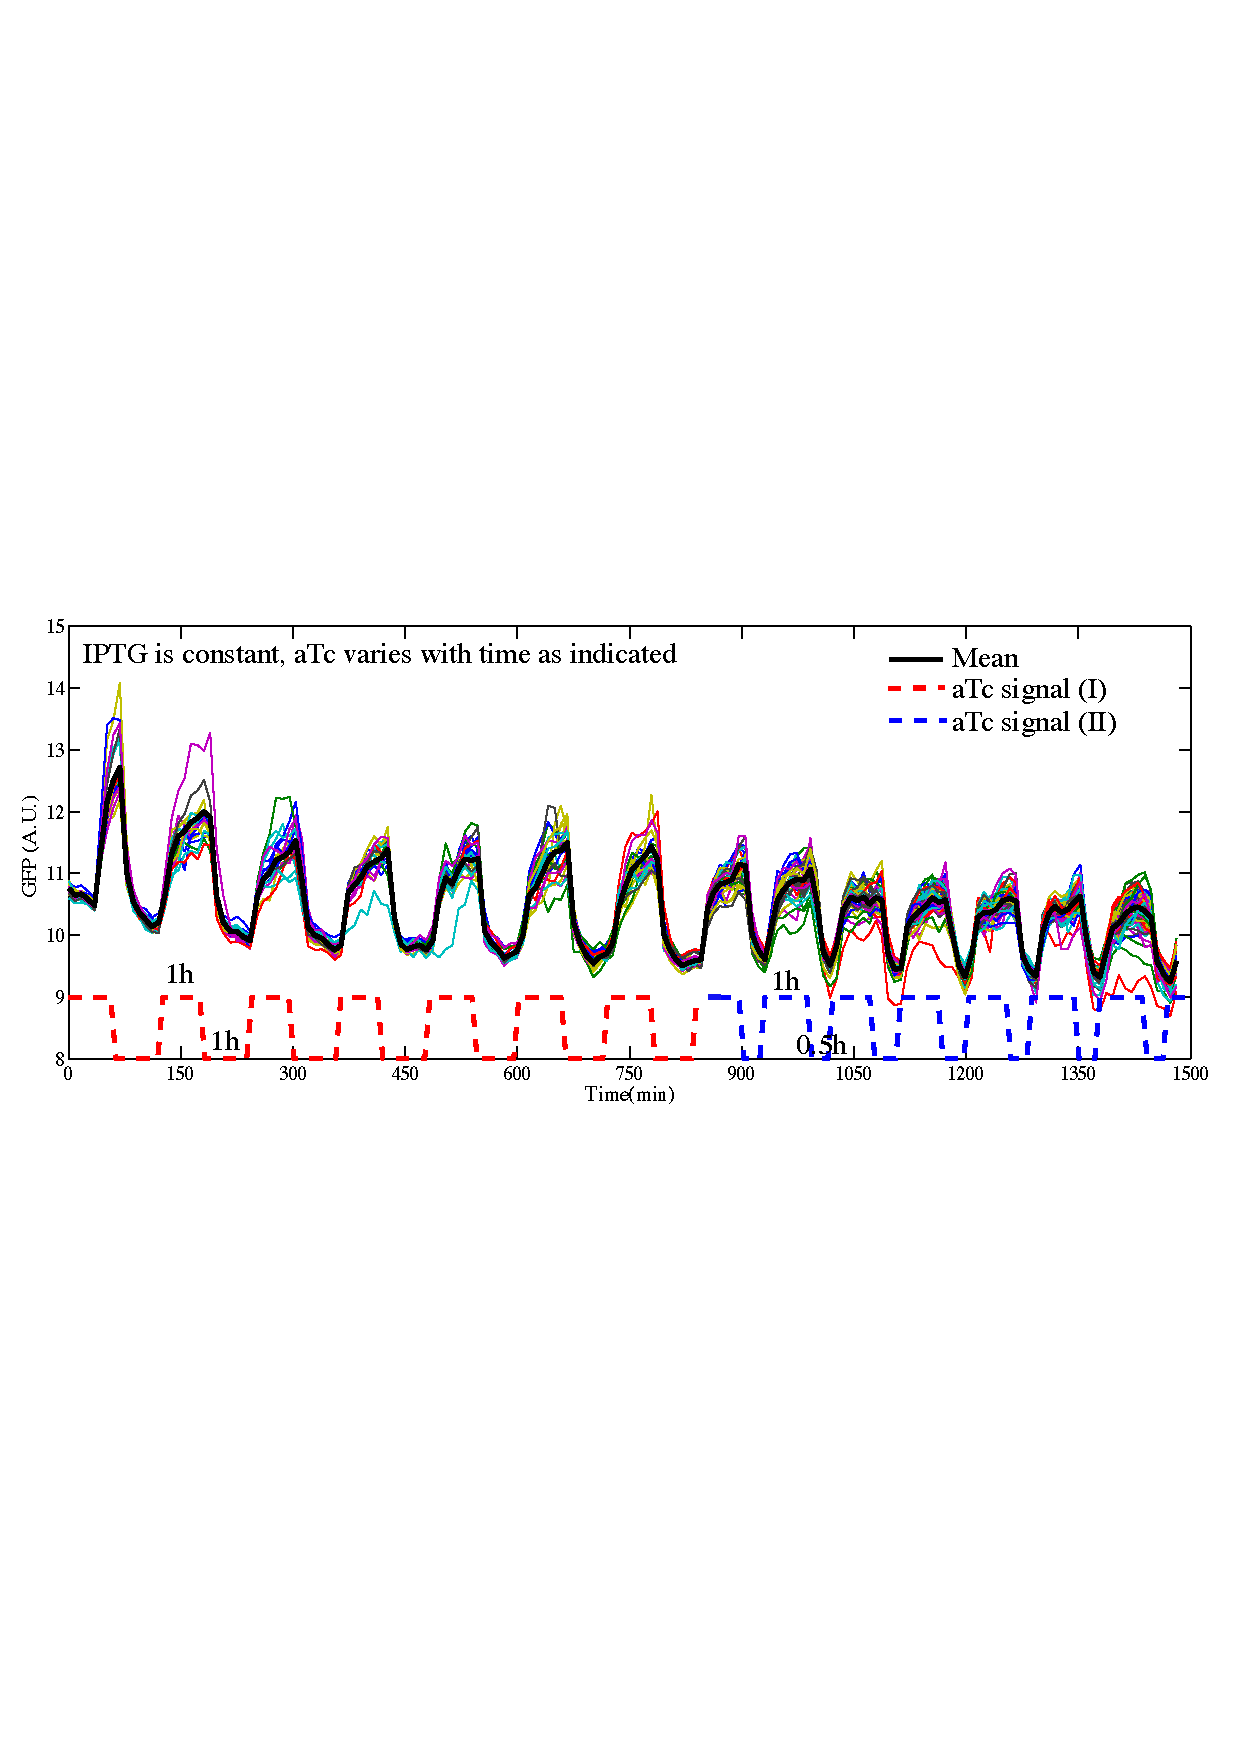
\includegraphics[trim = 0 310 0 300 , scale = 0.5, clip = true]{13_9}
\caption{The \textit{13\_9} dataset, with aTc forcing shown. IPTG concentration is constant at a level which saturates the cell's response. Note the forcing curve's height is schematic - aTc concentation is switched between off, and a level which saturates the cell's response}
\label{reactionscheme}
\end{figure}

%trim=l b r t
\begin{figure}[h]
\centering
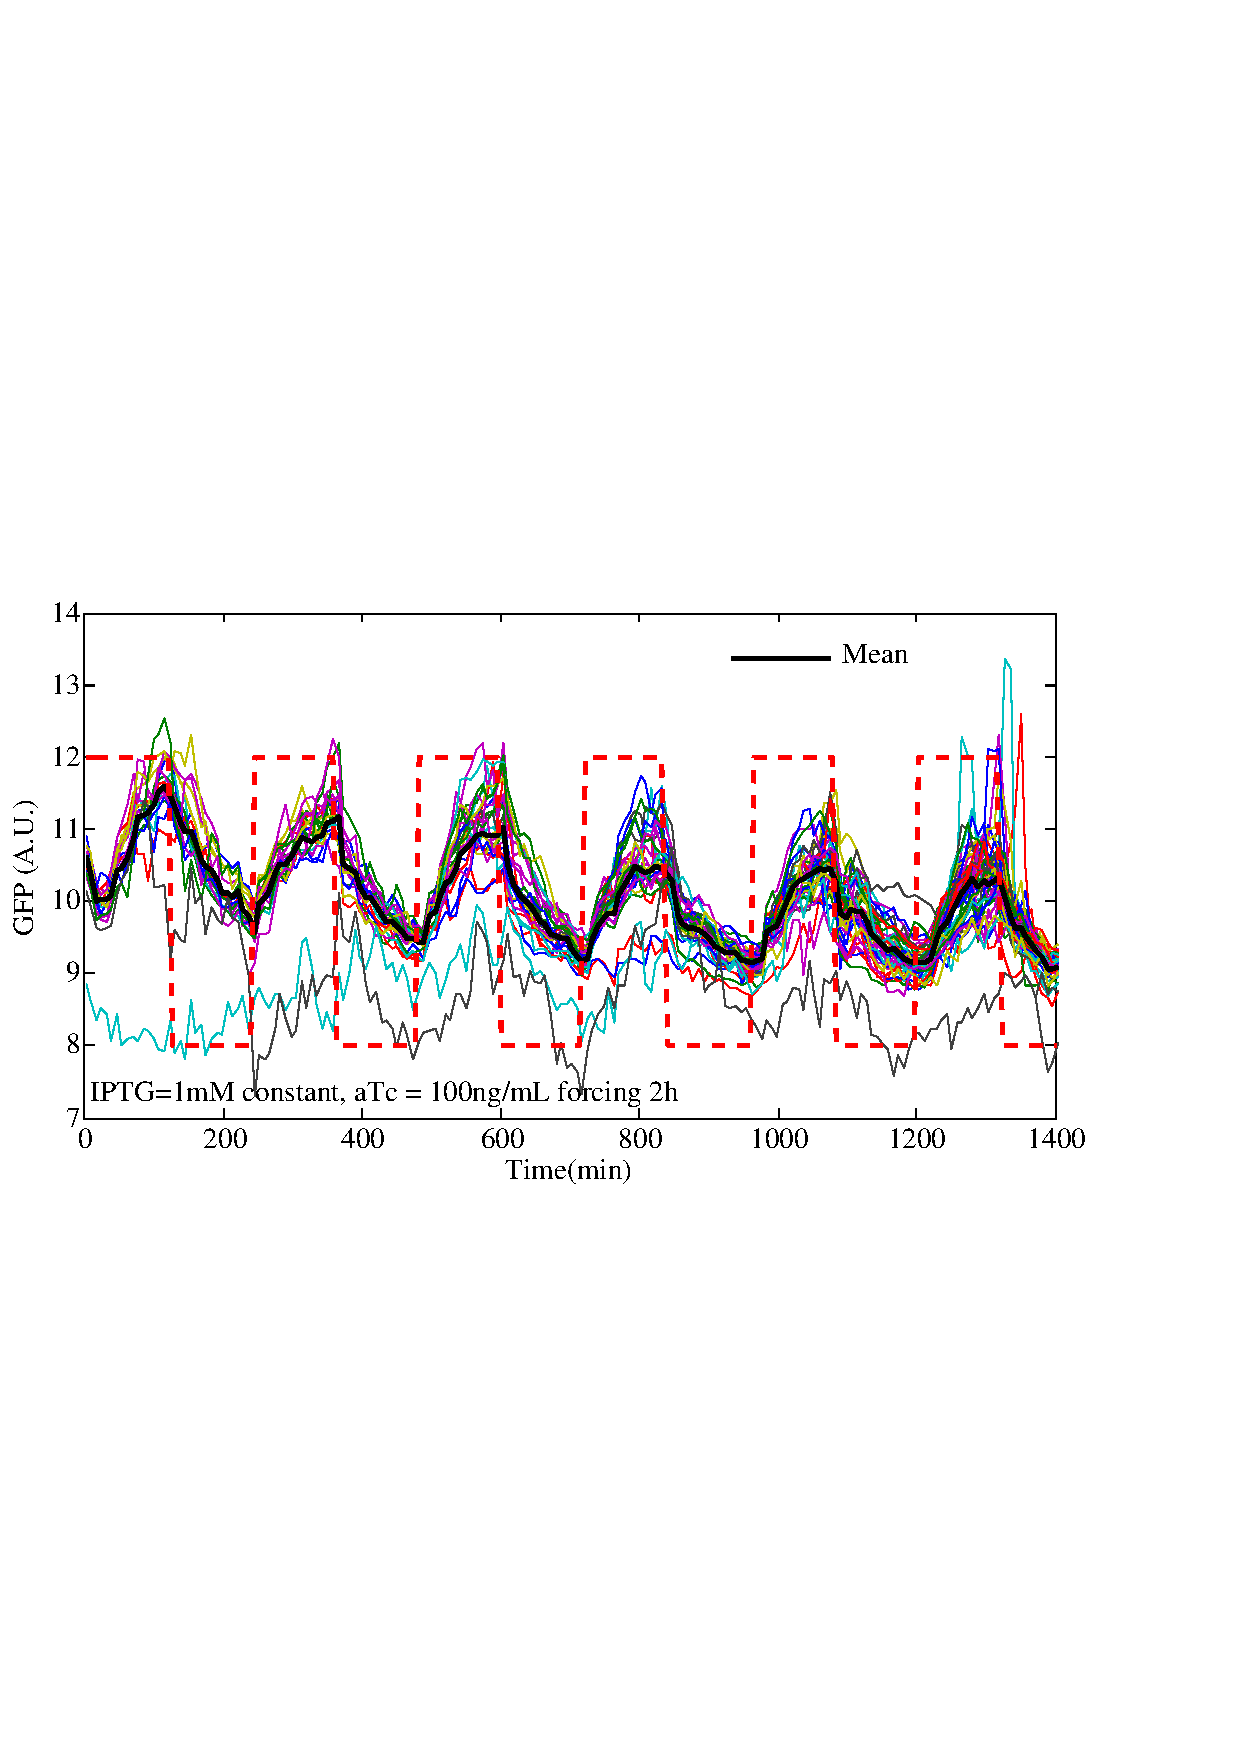
\includegraphics[trim = 0 270 0 360 , scale = 0.5, clip = true]{14_7}
\caption{The \textit{14\_7} dataset, with aTc forcing shown. IPTG concentration is constant at a level which saturates the cell's response. Note the forcing curve's height is schematic - aTc concentation is switched between off, and a level which saturates the cell's response}
\label{reactionscheme}
\end{figure}


\begin{figure}[h]
\centering
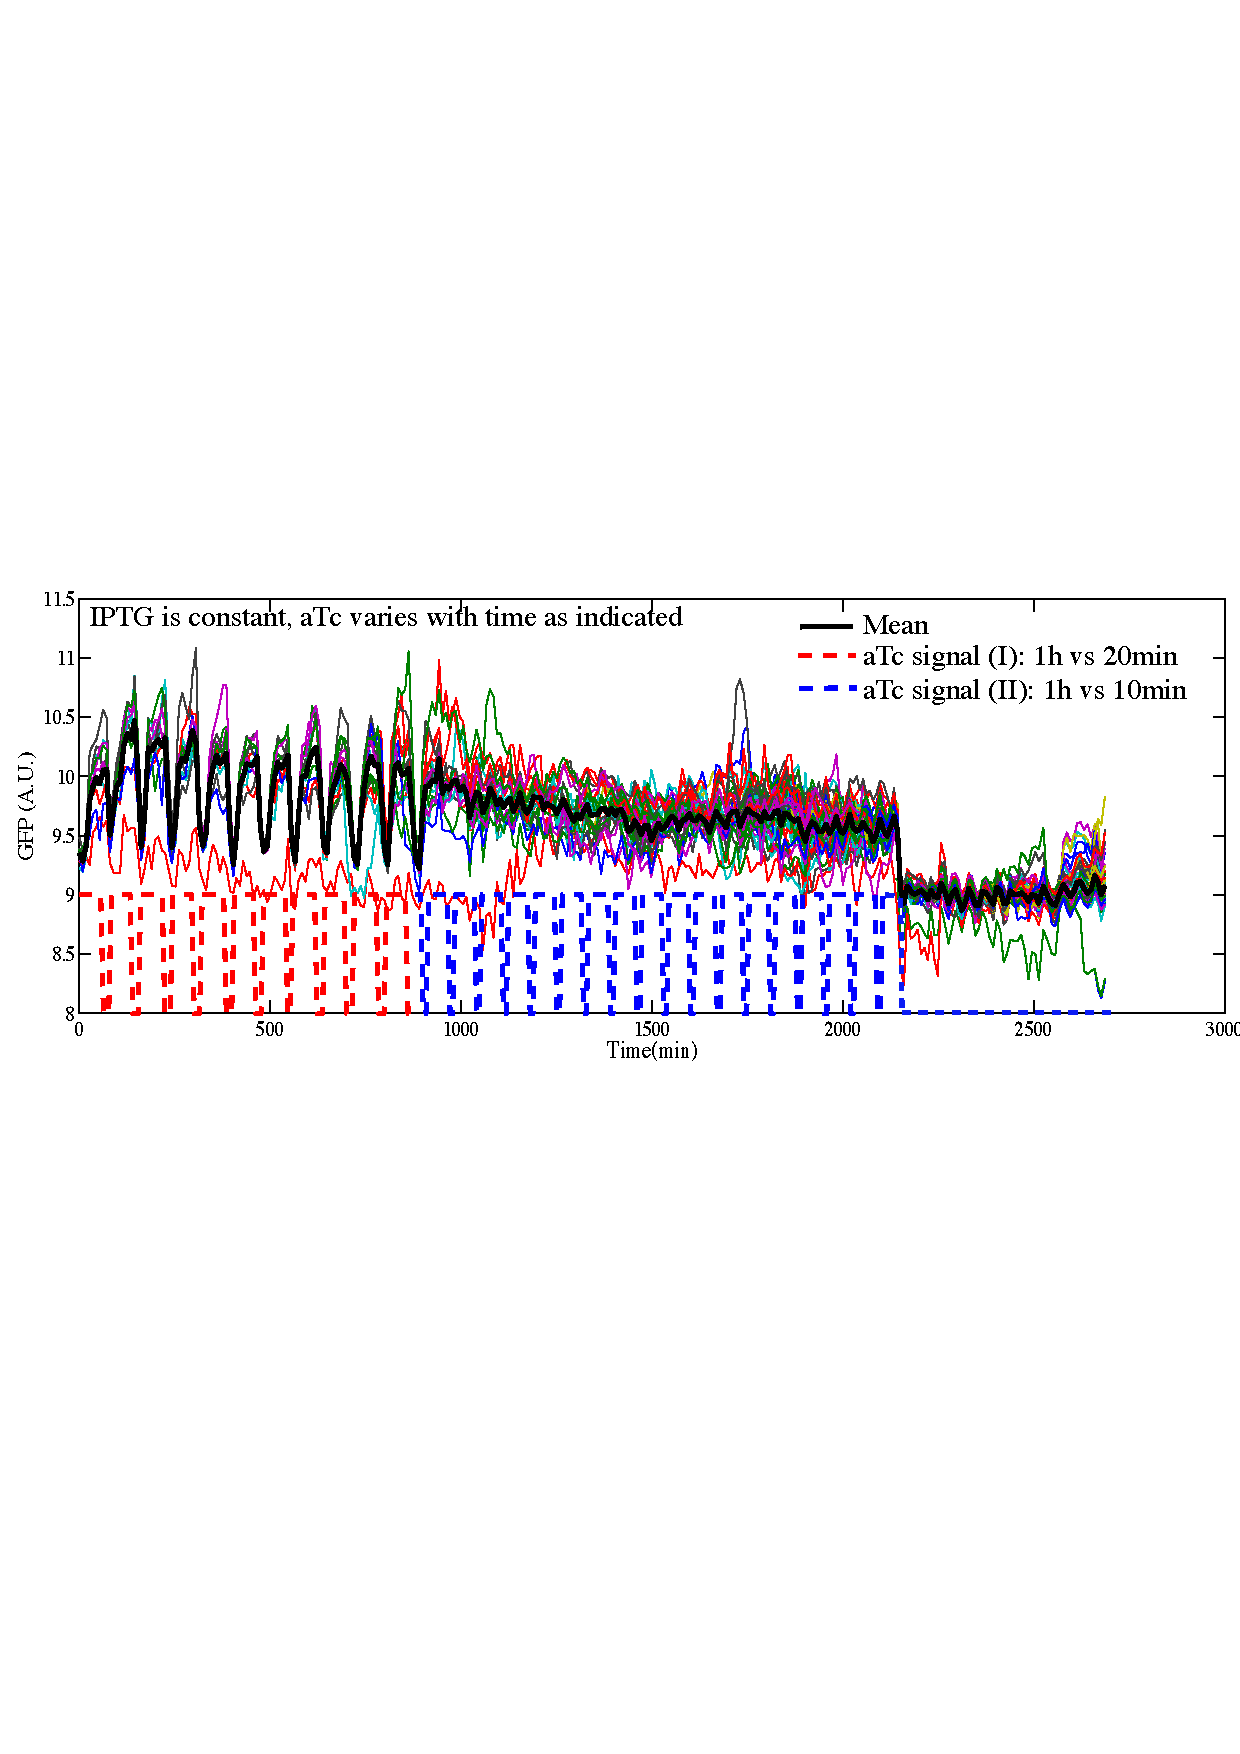
\includegraphics[trim = 0 330 0 270 , scale = 0.5, clip = true]{14_9}
\caption{The \textit{14\_9} dataset, with aTc forcing shown. IPTG concentration is constant at a level which saturates the cell's response. Note the forcing curve's height is schematic - aTc concentation is switched between off, and a level which saturates the cell's response}
\label{reactionscheme}
\end{figure}


\section{Histogram of Initial Fit Error values}
\label{Initial fit Error}
\setcounter{figure}{0}    

\begin{figure}[H]
    \begin{subfigure}[c]{\textwidth}
    \centering
        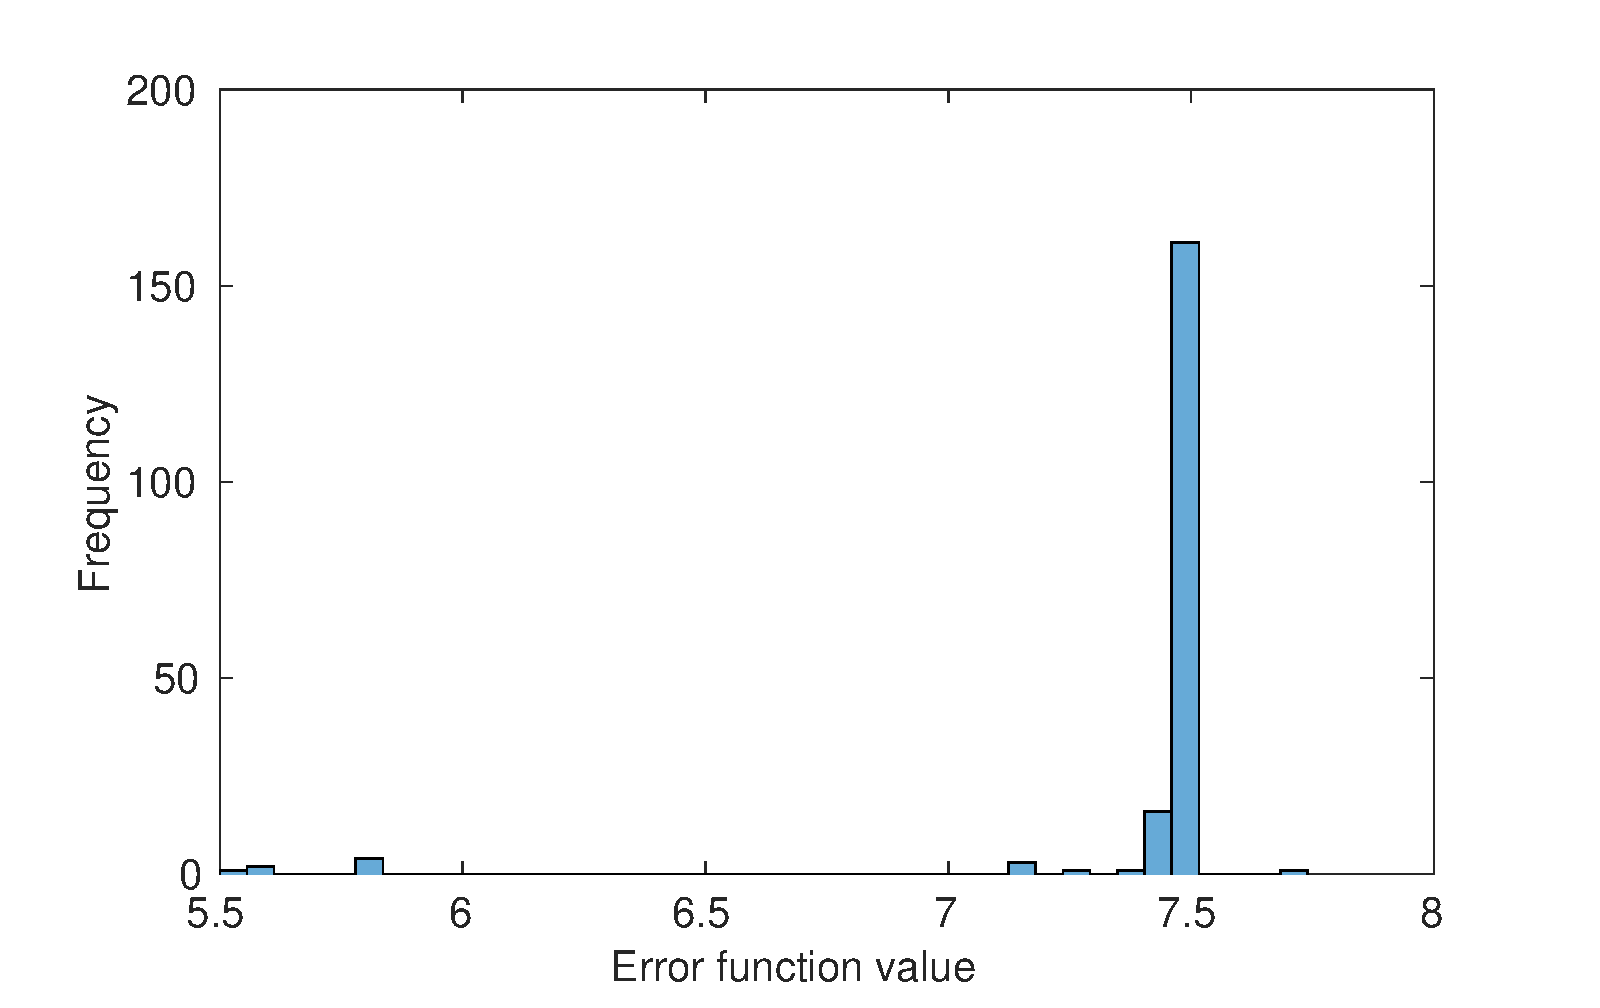
\includegraphics[scale = 0.5]{13_9_f_hist}
        \caption{Error values found from 200 initial parameter estimates, \textit{13\_9 dataset}.}
    \end{subfigure}
    
    \begin{subfigure}[c]{\textwidth}
    \centering
        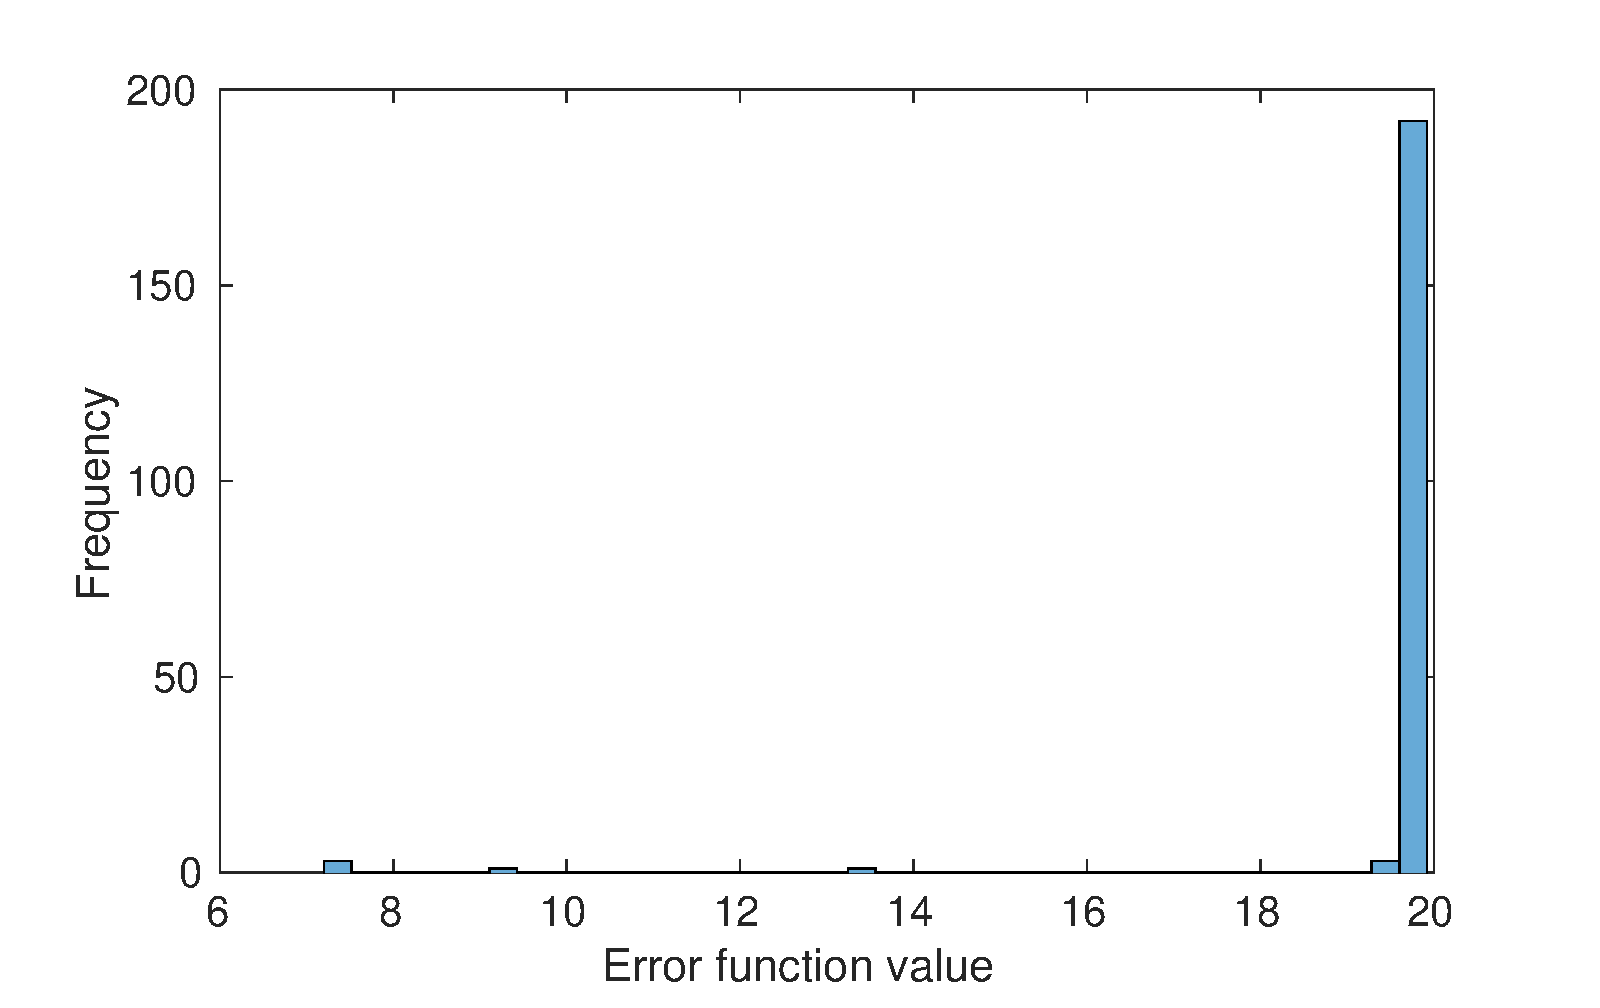
\includegraphics[scale = 0.5]{14_7_f_hist}
        \caption{Error values found from 200 initial parameter estimates, \textit{14\_7 dataset}}
    \end{subfigure}
    \caption{}
\label{hist_f}
\end{figure} 


\section{Parameter literature review}
\label{Parameter literature review}
\setcounter{figure}{0}    


\begin{table}[H]
\renewcommand{\arraystretch}{1.3}
\caption{Literature references, or initial rough bounds, on parameter values, with those to be estimated shown in bold}
\centering
\begin{tabular}{| l | l | p{0.3\linewidth} | p{0.1\linewidth} | p{0.1\linewidth} |}
\hline \textbf{Parameter} &  \textbf{Value} & \textbf{Definition} & \textbf{Reference} & \textbf{Initial Bounds}  \\
\hline \hline N & 300 & Number of copies of promoter existing on plasmid DNA & Experimentally set & \\
\hline $z_{0}$ &   9 AFU & Baseline experimental fluorescence & Experimentally determined &  \\
\hline $\alpha_{L}$ & 11 nM/min & Maximal transcription rate of $P_\mathrm{LlacO-1}$ promoter & \cite{Lutz1997} &\\
\hline $\alpha_{T}$  & 11 nM/min  & Maximal transcription rate of $P_{\mathrm{LtetO-1}}$ promoter  & \cite{Lutz1997}& \\
\hline $f_{L}$ & 620 & Unitless ratio between repressed and unrepressed $P_\mathrm{LlacO-1}$ transcription rate  & \cite{Lutz1997}  &  \\ 
\hline $f_{T}$ & 2535 & Unitless ratio between repressed and unrepressed $P_{\mathrm{LtetO-1}}$ transcription rate   & \cite{Lutz1997} &\\
\hline $\delta_{g}$  & 0.0005 /min  & GFP degradation rate & \cite{Andersen1998} &\\
\hline $\gamma$ &  0.132 /min & GFP maturation rate & \cite{Iizuka2011} & \\
\hline $v_{z}$ & 100 nM/min & degradation constant of clpx & \cite{Hersch2004} &\\
\hline $K_{z}$   &   75 nM/min & Dissociation constant of clpx & \cite{Hersch2004} &\\
\hline $\boldsymbol{\Theta}$  &   nM/AFU & Ratio between GFP concentration and observed fluoresence & & 300 - 1000  \\
\hline $\boldsymbol{\mu}$ &  /min & Dilution rate & & 0.001-0.05\\
\hline $\boldsymbol{\delta_{m}}$ &  /min & mRNA degredation rate & & 1 - $10^5$ \\
\hline $\boldsymbol{\delta_{s}}$ &  /min & sRNA degredation rate & & 1 - $10^3$ \\
\hline $\delta_{sm}$ &  /min & Unstable sRNA:mRNA degradation rate & &  Set to $\delta_m$\\
\hline $\delta_{c}$ &  /min & Stable sRNA:mRNA degradation rate & & Set to $\delta_m$ \\
\hline $\boldsymbol{k_{on}}$ &   /min & sRNA:mRNA binding rate & & 100 - $10^7$\\
\hline $\boldsymbol{k_{off}}$ &  /min & sRNA:mRNA unbinding rate & & 1 -$10^8$\\
\hline $\boldsymbol{k_{hyb}}$ &  /min & sRNA:mRNA hybridization rate & & 1 - $10^4$ \\
\hline $\boldsymbol{\beta}$ &   /min & Baseline translation rate of repressed mRNA & & 0.0001 - 10\\
\hline $\boldsymbol{f_{s}}$ & & Ratio of repressed mRNA to unrepressed complex translation rate. & & 0.1 - $10^4$\\
\hline
\end{tabular}
\end{table}




\end{document}